\documentclass{beamer}
\beamertemplatenavigationsymbolsempty

\mode<presentation>
{
  \usetheme{Madrid}
  \usecolortheme{seahorse}
  \setbeamercovered{transparent}
}
\usepackage{graphicx}
\usepackage[english]{babel}
\usepackage[latin1]{inputenc}
\usepackage{times}
\usepackage[T1]{fontenc} 
% Or whatever. Note that the encoding and the font should match. If T1
% does not look nice, try deleting the line with the fontenc.
\usepackage{amsmath}
\usepackage{color}
\newcommand{\linespace}{\vskip 0.25cm}
\usepackage{rotating}

\definecolor{MyForestGreen}{rgb}{0,0.7,0} 
\newcommand{\tableemph}[1]{{#1}}
\newcommand{\tablewin}[1]{\tableemph{#1}}
\newcommand{\tablemid}[1]{\tableemph{#1}}
\newcommand{\tablelose}[1]{\tableemph{#1}}

\definecolor{MyLightGray}{rgb}{0.6,0.6,0.6}
\newcommand{\tabletie}[1]{\color{MyLightGray} {#1}}

% The text in square brackets is the short version of your title and will be used in the
% header/footer depending on your theme.
\title[Visualizing Genetic Programming Ancestries]{Visualizing Genetic Programming Ancestries}

% Sub-titles are optional - uncomment and edit the next line if you want one.
% \subtitle{Why does sub-tree crossover work?} 

% The text in square brackets is the short version of your name(s) and will be used in the
% header/footer depending on your theme.
\author[McPhee \& Casale]{McPhee\inst{1}, Casale\inst{2}, Finzel, Helmuth, \& Spector}

% The text in square brackets is the short version of your institution and will be used in the
% header/footer depending on your theme.
\institute[]
{
	\inst{1} Division of Science and Mathematics \\
	University of Minnesota, Morris \\
	Morris, Minnesota, USA \and %
	\inst{2} Design Center Inc. \\
	St. Paul, Minnesota, USA}

% The text in square brackets is the short version of the date if you need that.
\date[July '16, VizGEC] % (optional)
{21 July 2016 \\ VizGEC}

% Delete this, if you do not want the table of contents to pop up at
% the beginning of each subsection:
\AtBeginSection[]
{
  \begin{frame}<beamer>
    \frametitle{Outline}
    \tableofcontents[currentsection, hideothersubsections]
  \end{frame}
}

\begin{document}

\begin{frame}
  \titlepage
\end{frame}

\section*{Overview}




\subsection*{Why?}

\begin{frame}{Why?}	
\begin{columns}
% Column 1
\begin{column}{0.6\textwidth}
%Look at Into. from paper with David last year.
Evolutionary Computation allows us to:
\begin{itemize}
\item Create algorithmic solutions by simulating biological evolution.
\item Derive solutions that humans wouldn't necessarily find.
\begin{itemize}
\item Like NASA's antenna! $\rightarrow$
\end{itemize}
\end{itemize}
\vspace{.5cm}
Our Research has allowed us to:
\begin{itemize}
\item Turn our complex runs into organized ancestry trees.
\item Modify aspects of both nodes and edges to visualize analytics.
\item Find patterns in data that couldn't be seen in previous work.
\end{itemize}
\end{column}
% Column 2
\begin{column}{0.3\textwidth}
\center 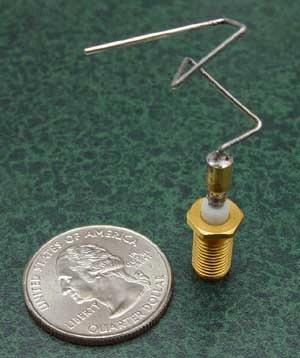
\includegraphics[width=\textwidth]{Illustrations/antenna.jpg}\\{\tiny \url{https://en.wikipedia.org/wiki/Evolved_antenna}}
\end{column}
\end{columns}
\end{frame}

\begin{frame}{Family Tree}
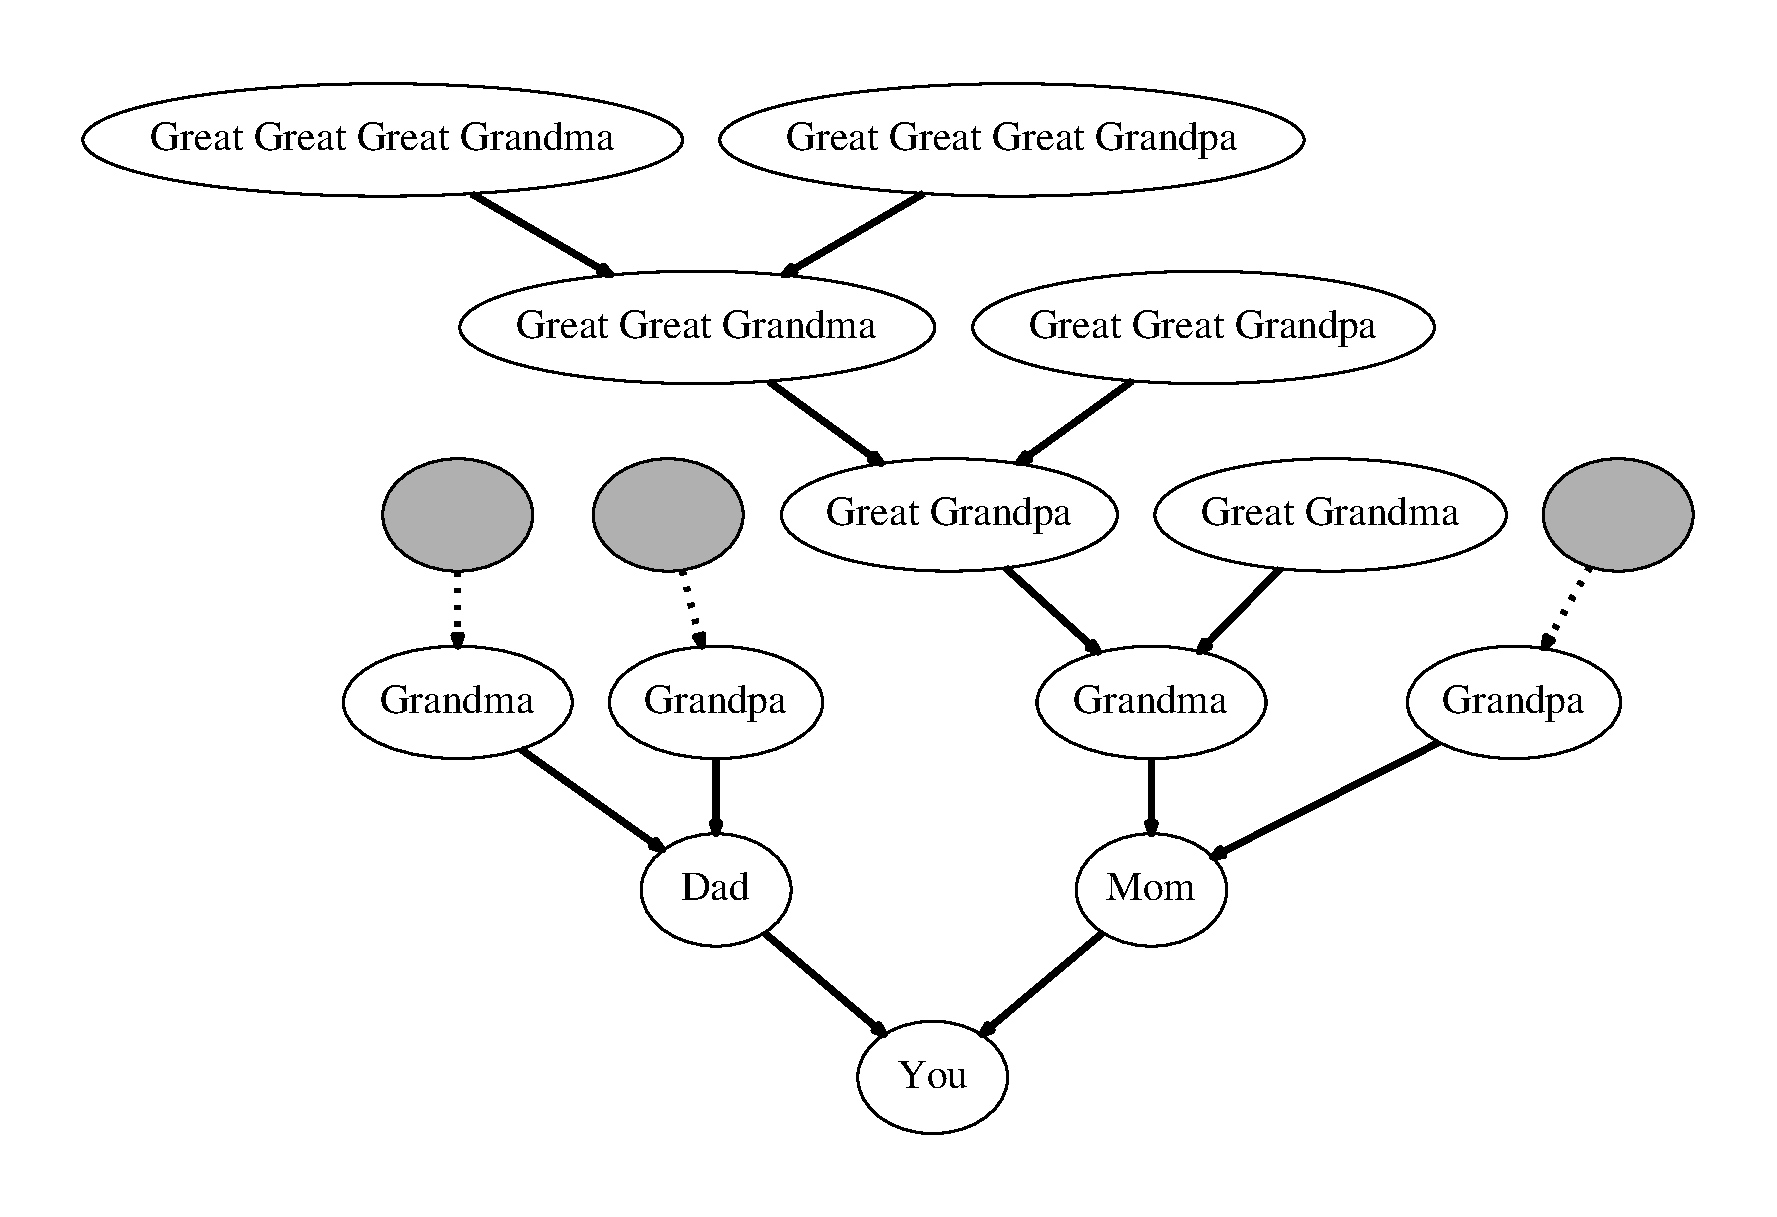
\includegraphics[width=\textwidth]{Illustrations/family_blank.pdf}
\end{frame}

\begin{frame}{Highlighted Individuals}
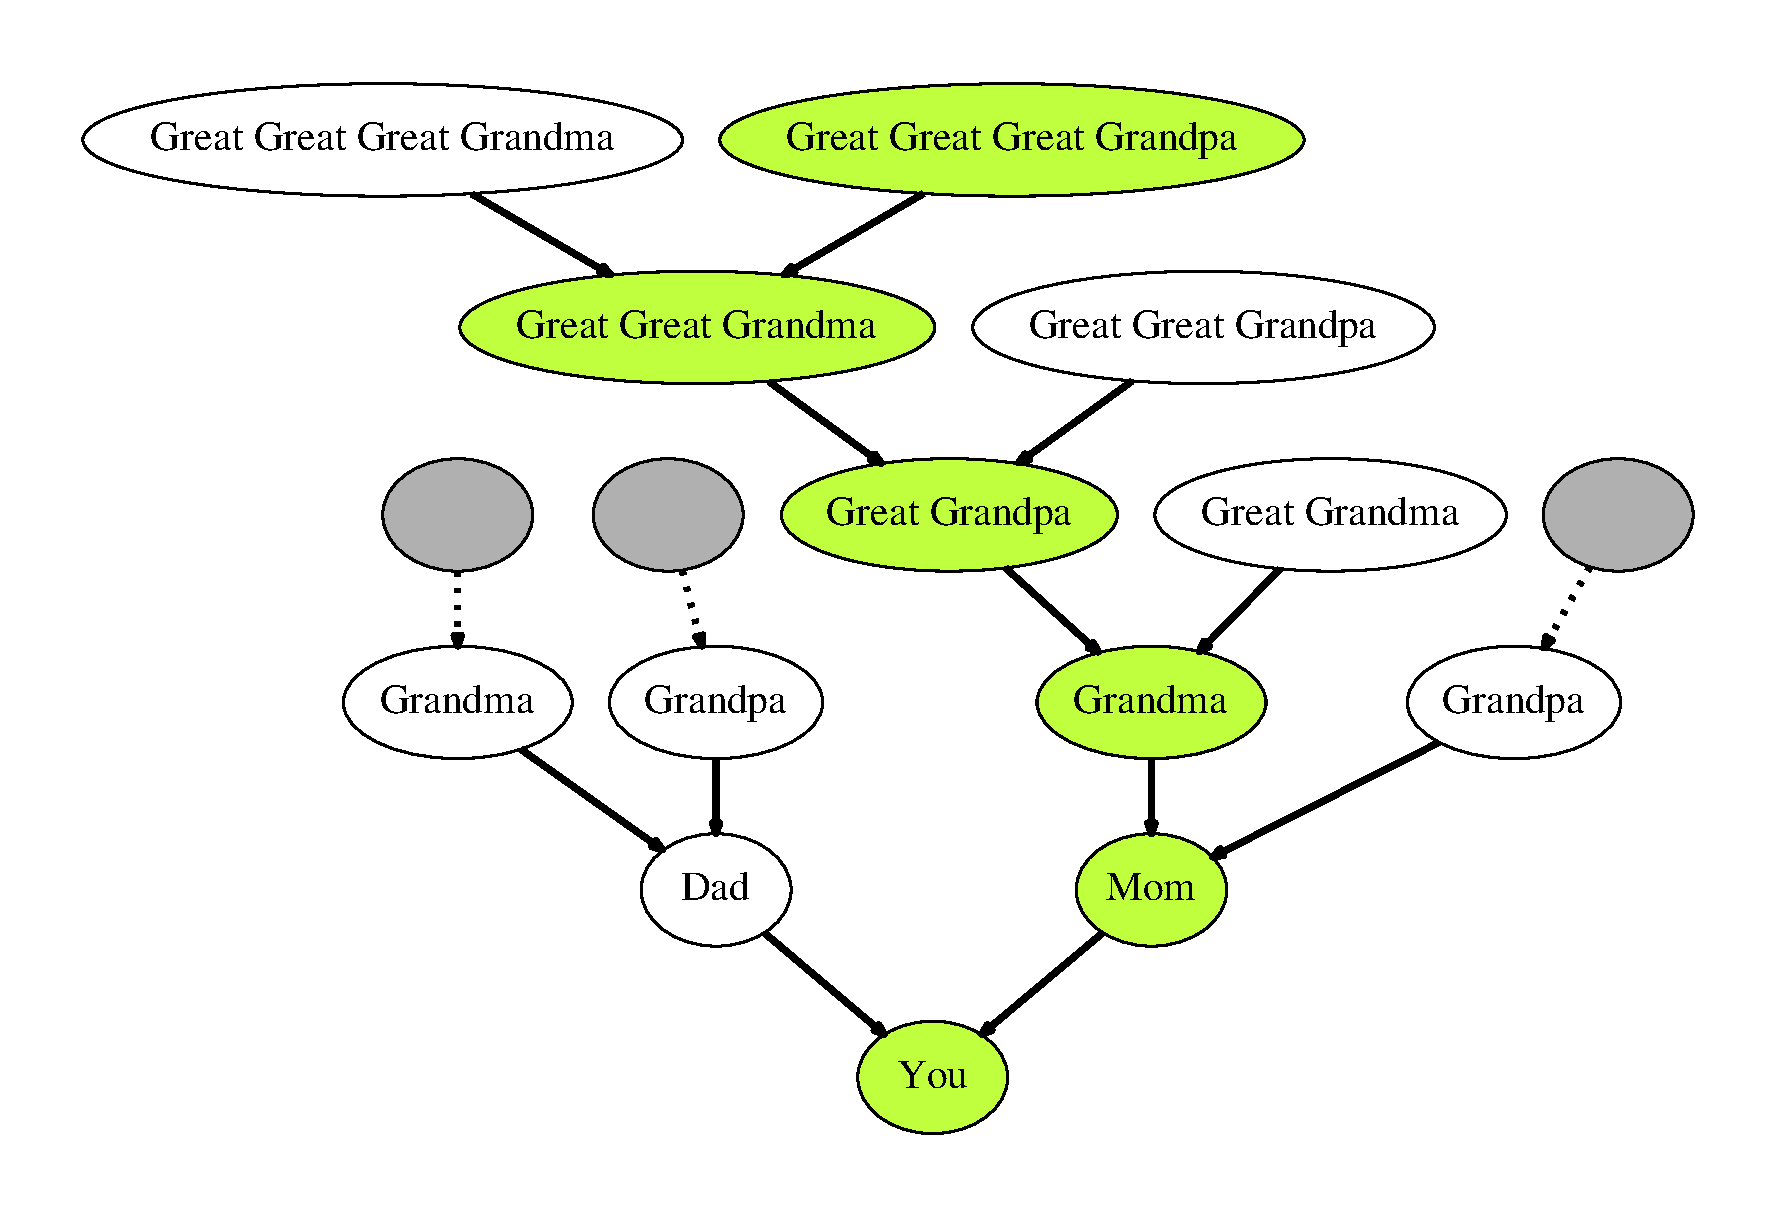
\includegraphics[width=\textwidth]{Illustrations/family_path.pdf} 
\end{frame}

\subsection*{Outline}

\begin{frame}{Outline}
  \tableofcontents[hideallsubsections]
\end{frame}

%~~~~~~~~~~Background~~~~~~~~~~~~~~~~~~~~~~~~~~~~~~~~~~~~~~~~~~~~~~~~~~~~~~~~~~~~~~~~~~~~~~~~~~~~~~~~~~~~~~~

\section[Background]{Background}

\subsection[Evolutionary Computation]{Evolutionary Computation}
\begin{frame}{Evolutionary Computation Versus Biological Evolution}
\center
\begin{columns}
%Column 1
\begin{column}[t]{0.4\textwidth}
Evolutionary Computation
\begin{itemize}
\item Programs
\item Population growth occurs until solution
\end{itemize}
\center 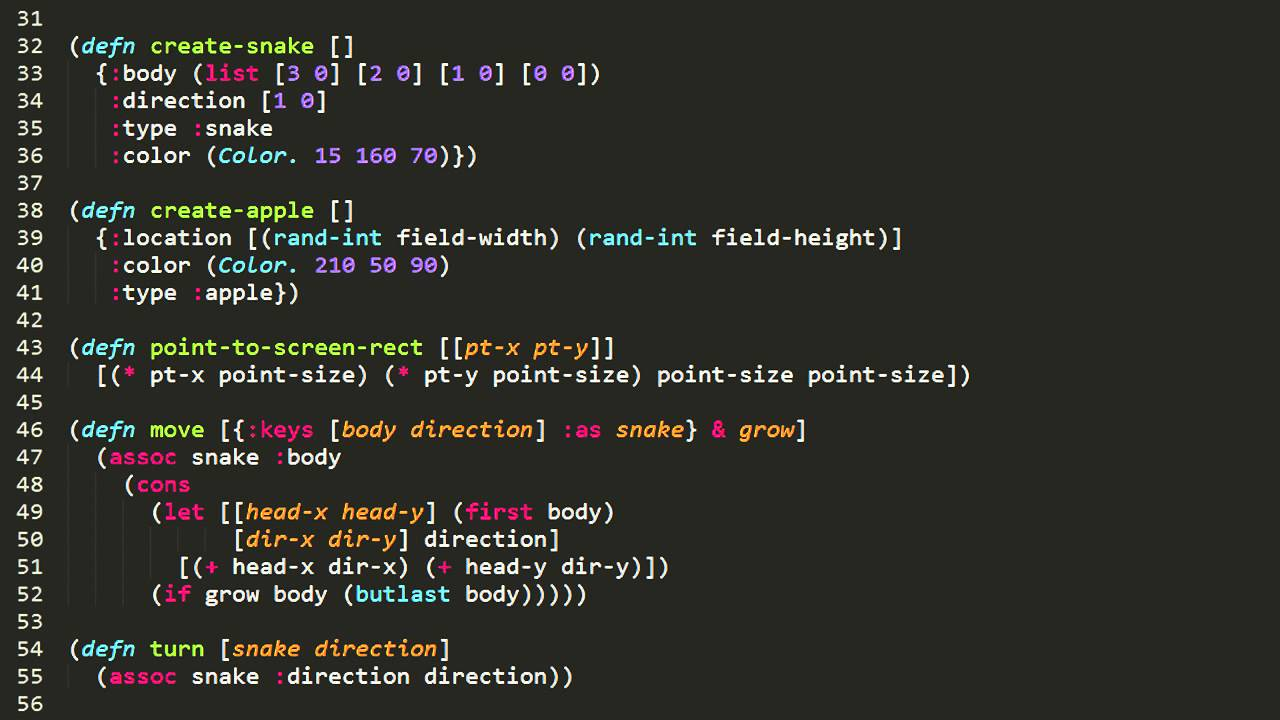
\includegraphics[width=\textwidth]{Illustrations/code.jpg}\\{\tiny \url{https://i.ytimg.com/vi/-XzSGPJRBsw/maxresdefault.jpg}}
\end{column}
%Column 2
\begin{column}[t]{0.4\textwidth}
Biological Evolution
\begin{itemize}
\item Organisms
\item Continuous growth 
\end{itemize}
\medskip
\center 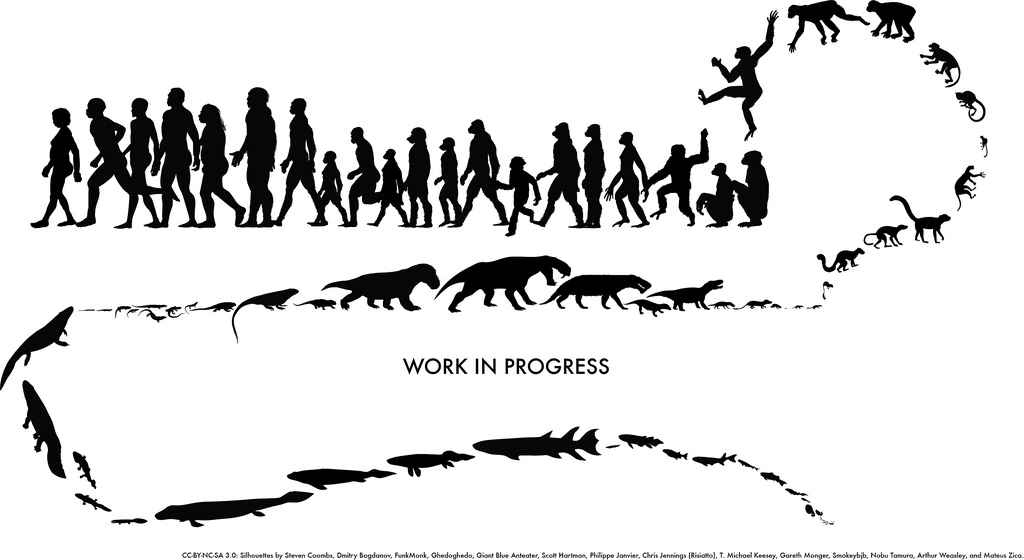
\includegraphics[width=\textwidth]{Illustrations/evolution.jpg}\\{\tiny \url{https://www.flickr.com/photos/keesey/9915333023}}
\end{column}
\end{columns}
\end{frame}

\subsection[Runs]{Runs}
\begin{frame}{Run Structure}
In a run, we have many generations of individuals or programs.
\begin{itemize}
\item Start with 1,000 individuals
\item Test each individual on 200 test cases
\item Assign error based on test results
\item If a solution is found, stop
\item Otherwise, make a new generation
\end{itemize} 
\end{frame}

\subsection[Ancestry Trees]{Ancestry Trees}
\begin{frame}{Ancestry Trees: Basic Structure}
\center 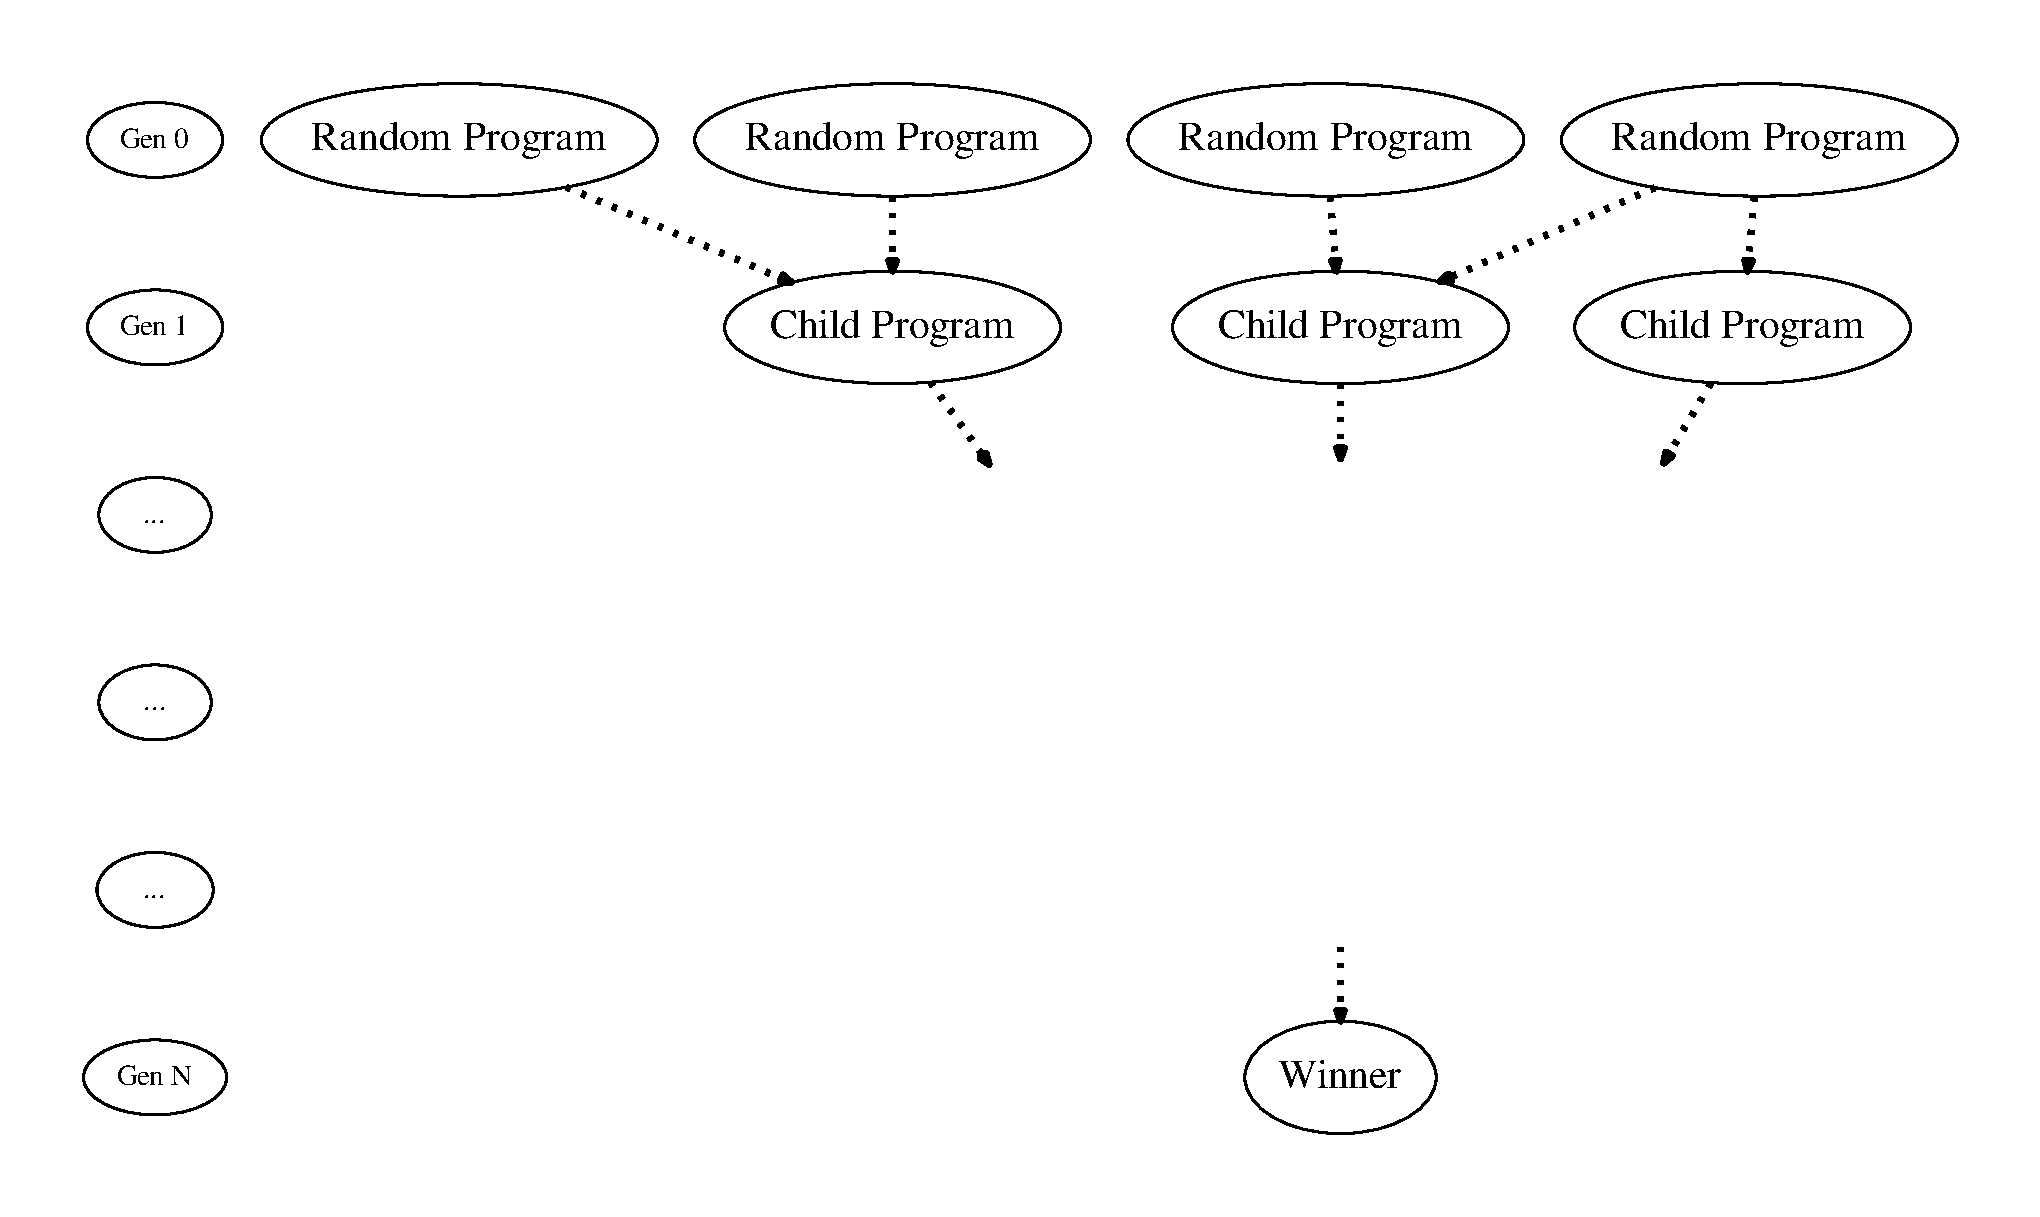
\includegraphics[width=\textwidth]{Illustrations/generic_run.pdf} 
\end{frame}

\begin{frame}{Basic Run 0}
\center Random Programs $\downarrow$ \\
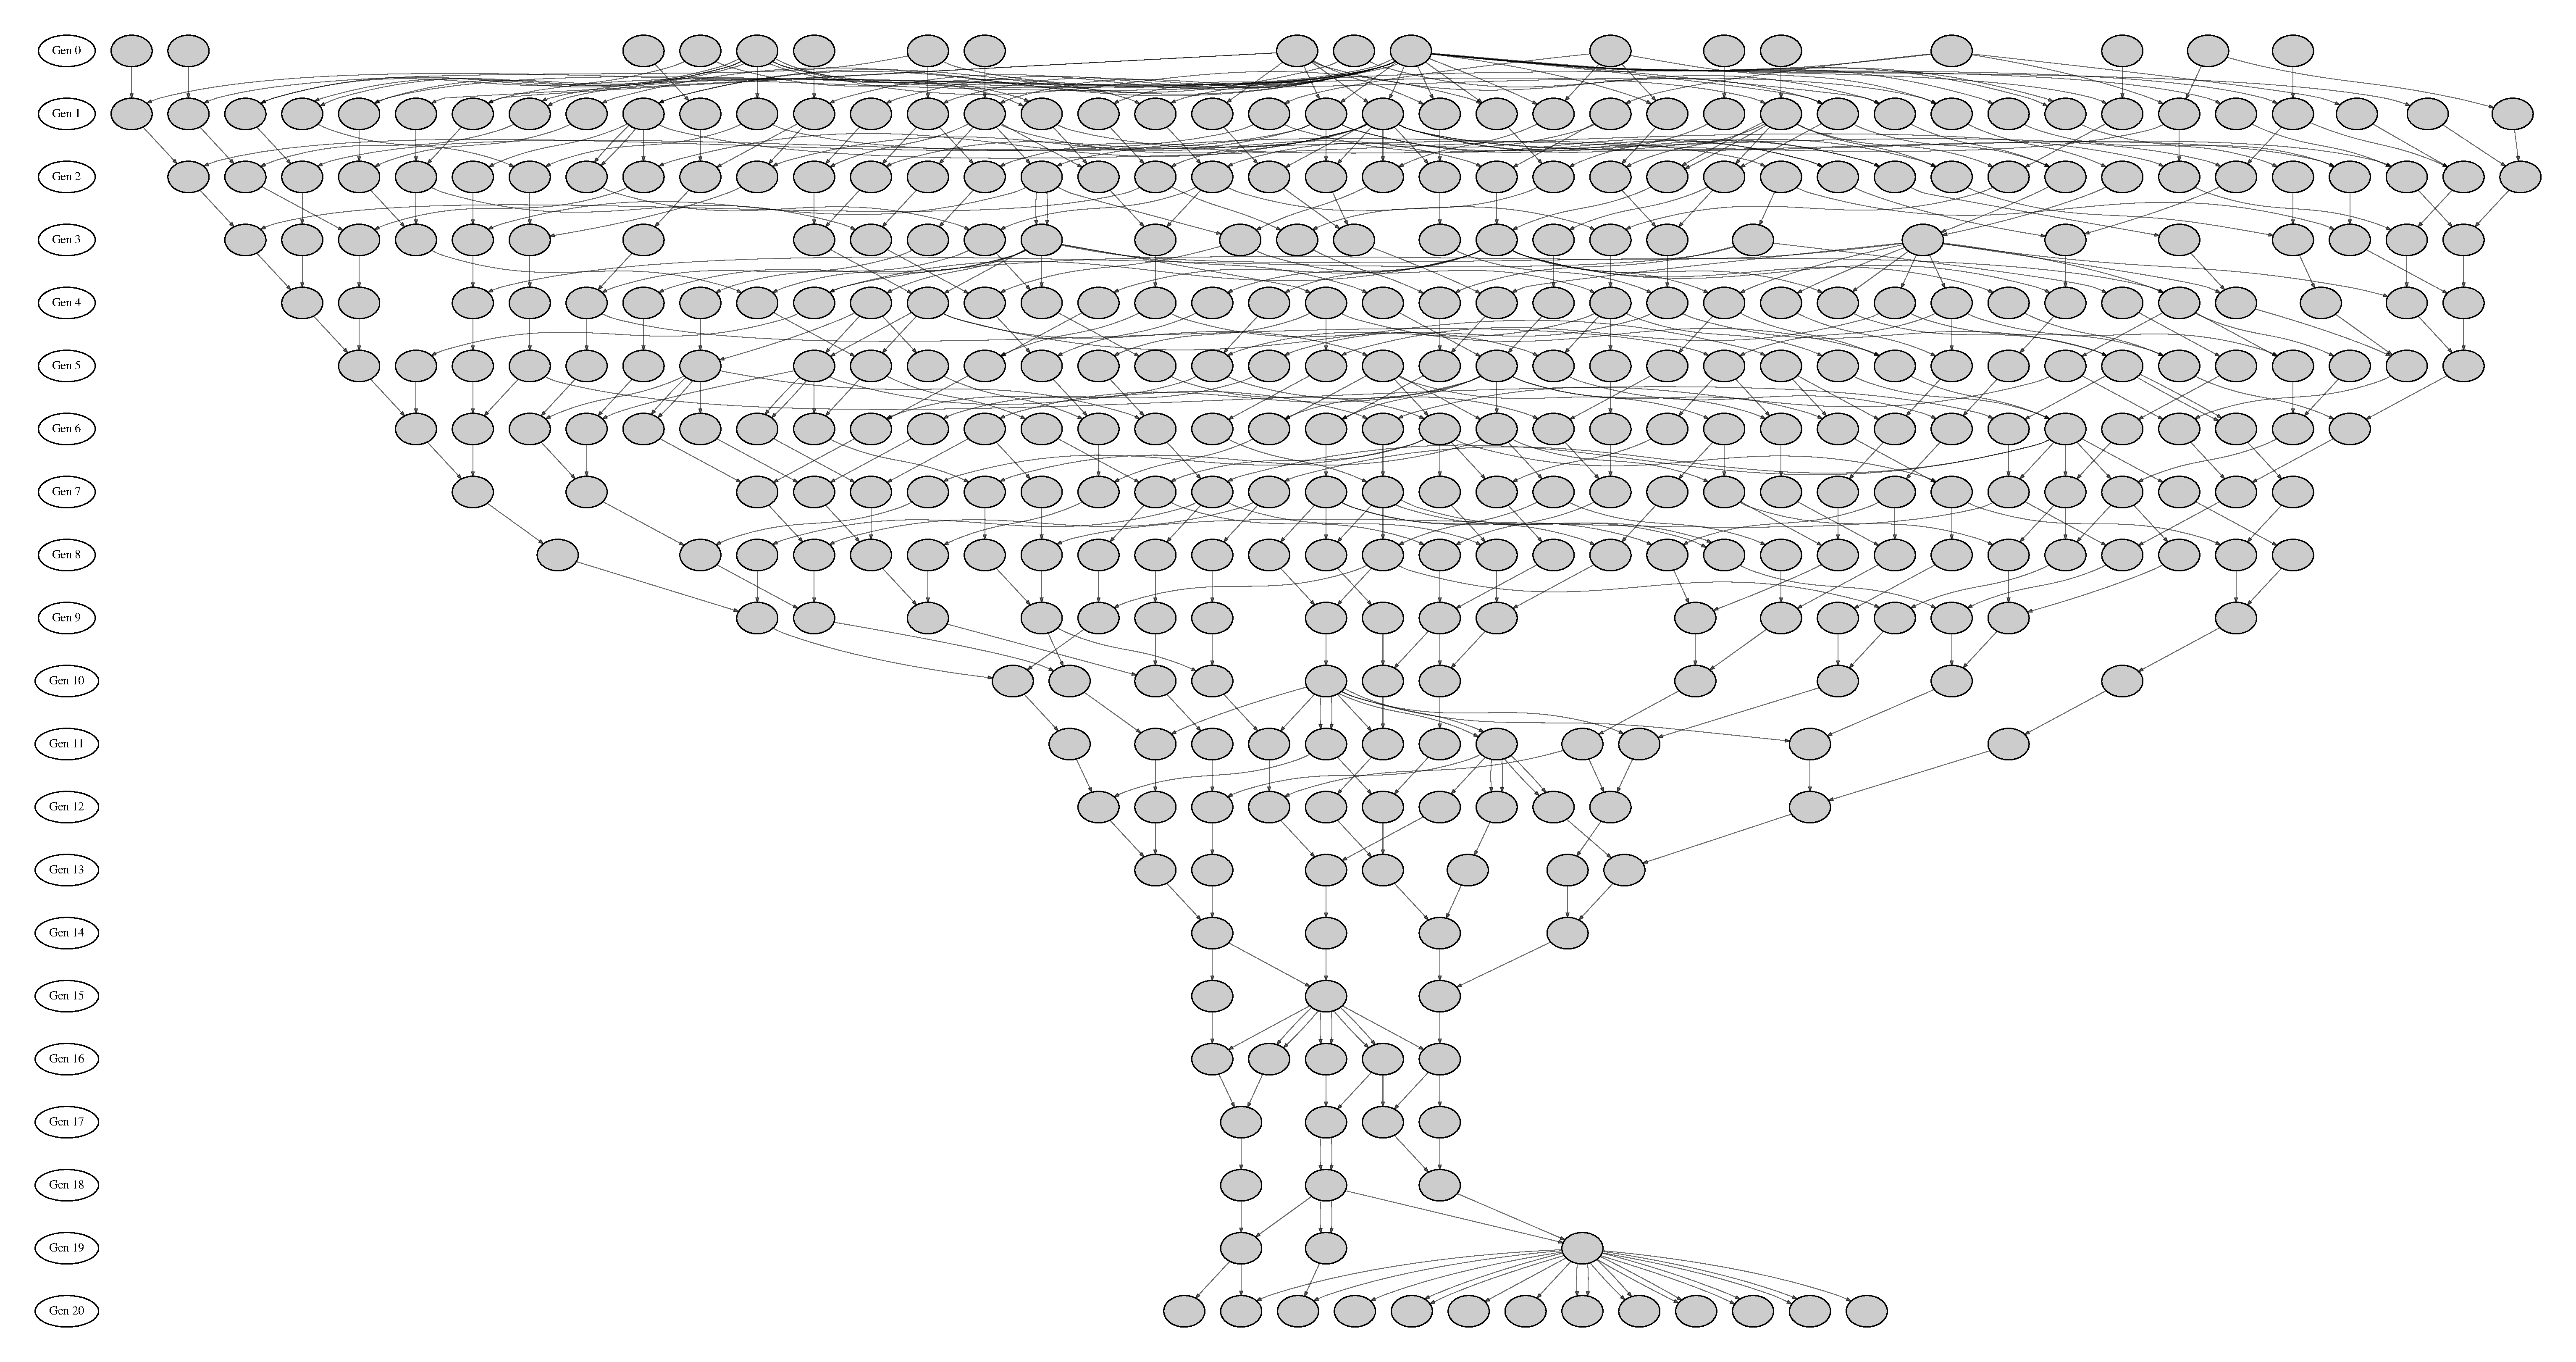
\includegraphics[width=\textwidth]{Illustrations/run0_basic_structure.pdf} \\
Winning Program(s) $\uparrow$ 
\end{frame}

%~~~~~~~~~~Graph Structure~~~~~~~~~~~~~~~~~~~~~~~~~~~~~~~~~~~~~~~~~~~~~~~~~~~~~~~~~~~~~~~~~~~~~~~~~~~~~~~~~~~~~~
\section{Graph Structure}

\subsection[Nodes]{Nodes}

\begin{frame}{Node Basics}
Nodes represent an individual or program.\\ They know:
\begin{itemize}
\item Number of selections: Width
\item Number of children: Height
\end{itemize}
\bigskip
\hspace{6.25cm} $\leftarrow$ Number of Selections $\rightarrow$
\begin{tabular}{rc}
\begin{tabular}{r}
\hspace{1cm} $\uparrow$ Number of Children $\downarrow$
\end{tabular}
\begin{tabular}{c}
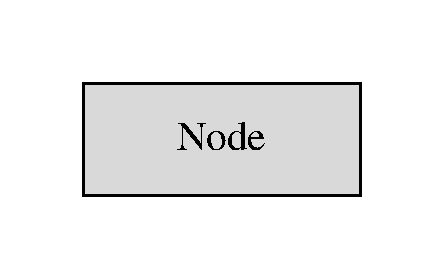
\includegraphics[width=.45\textwidth]{Illustrations/node_and_edge.pdf}
\end{tabular}
\end{tabular}
\end{frame}

\begin{frame}{Run 0: No color}
\center 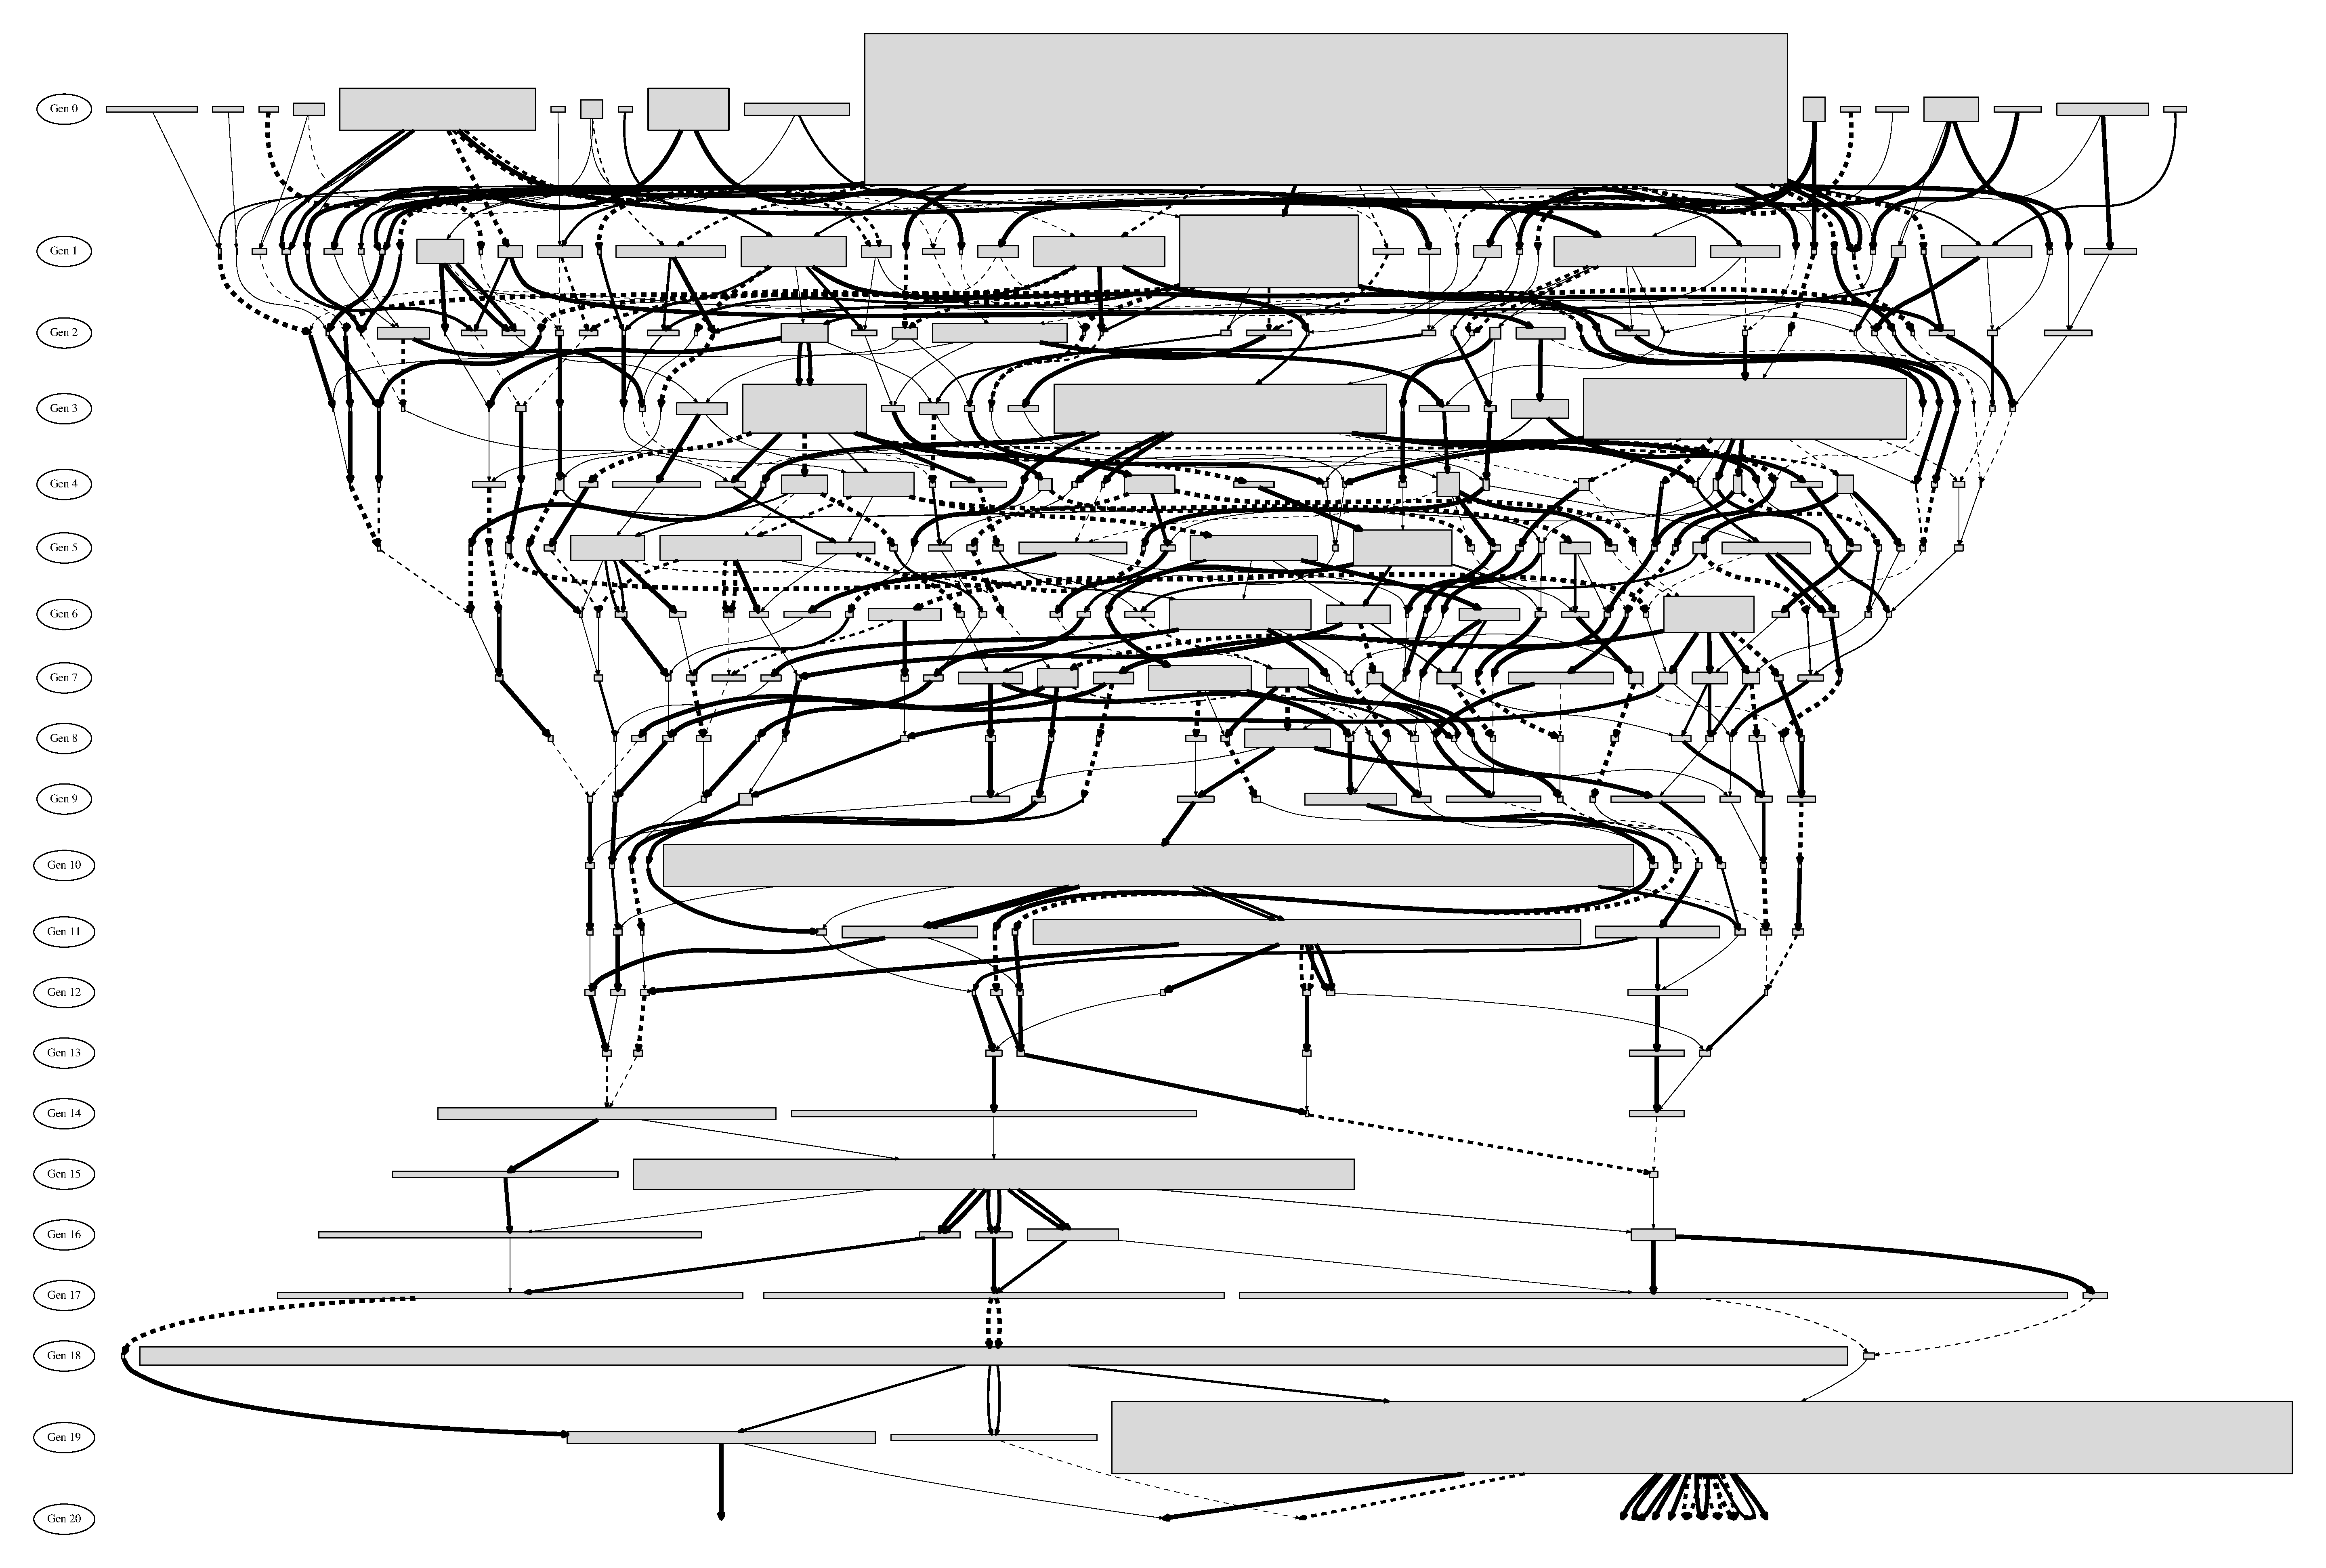
\includegraphics[width=.95\textwidth]{Illustrations/run0_no_color.pdf} 
\end{frame}

\begin{frame}{Node Coloring}
\center
{There are two different techniques we use:  \\ Error Based  \&  RBM}

\includegraphics[width=\textwidth]{Illustrations/run0_dual_and_RBM_full.pdf}
\end{frame}

\begin{frame}{Error Based Node Coloring}
\begin{columns}
% Column 1
\begin{column}{.4\textwidth}
\begin{itemize}
\item Two part problem
\item Based on an individual's total error.
\item Additional shading for very high errors.
\end{itemize}
\center

\includegraphics[height=0.4\textheight]{Illustrations/colorrange.pdf}
\end{column}
% Column 2
\begin{column}{.6\textwidth}
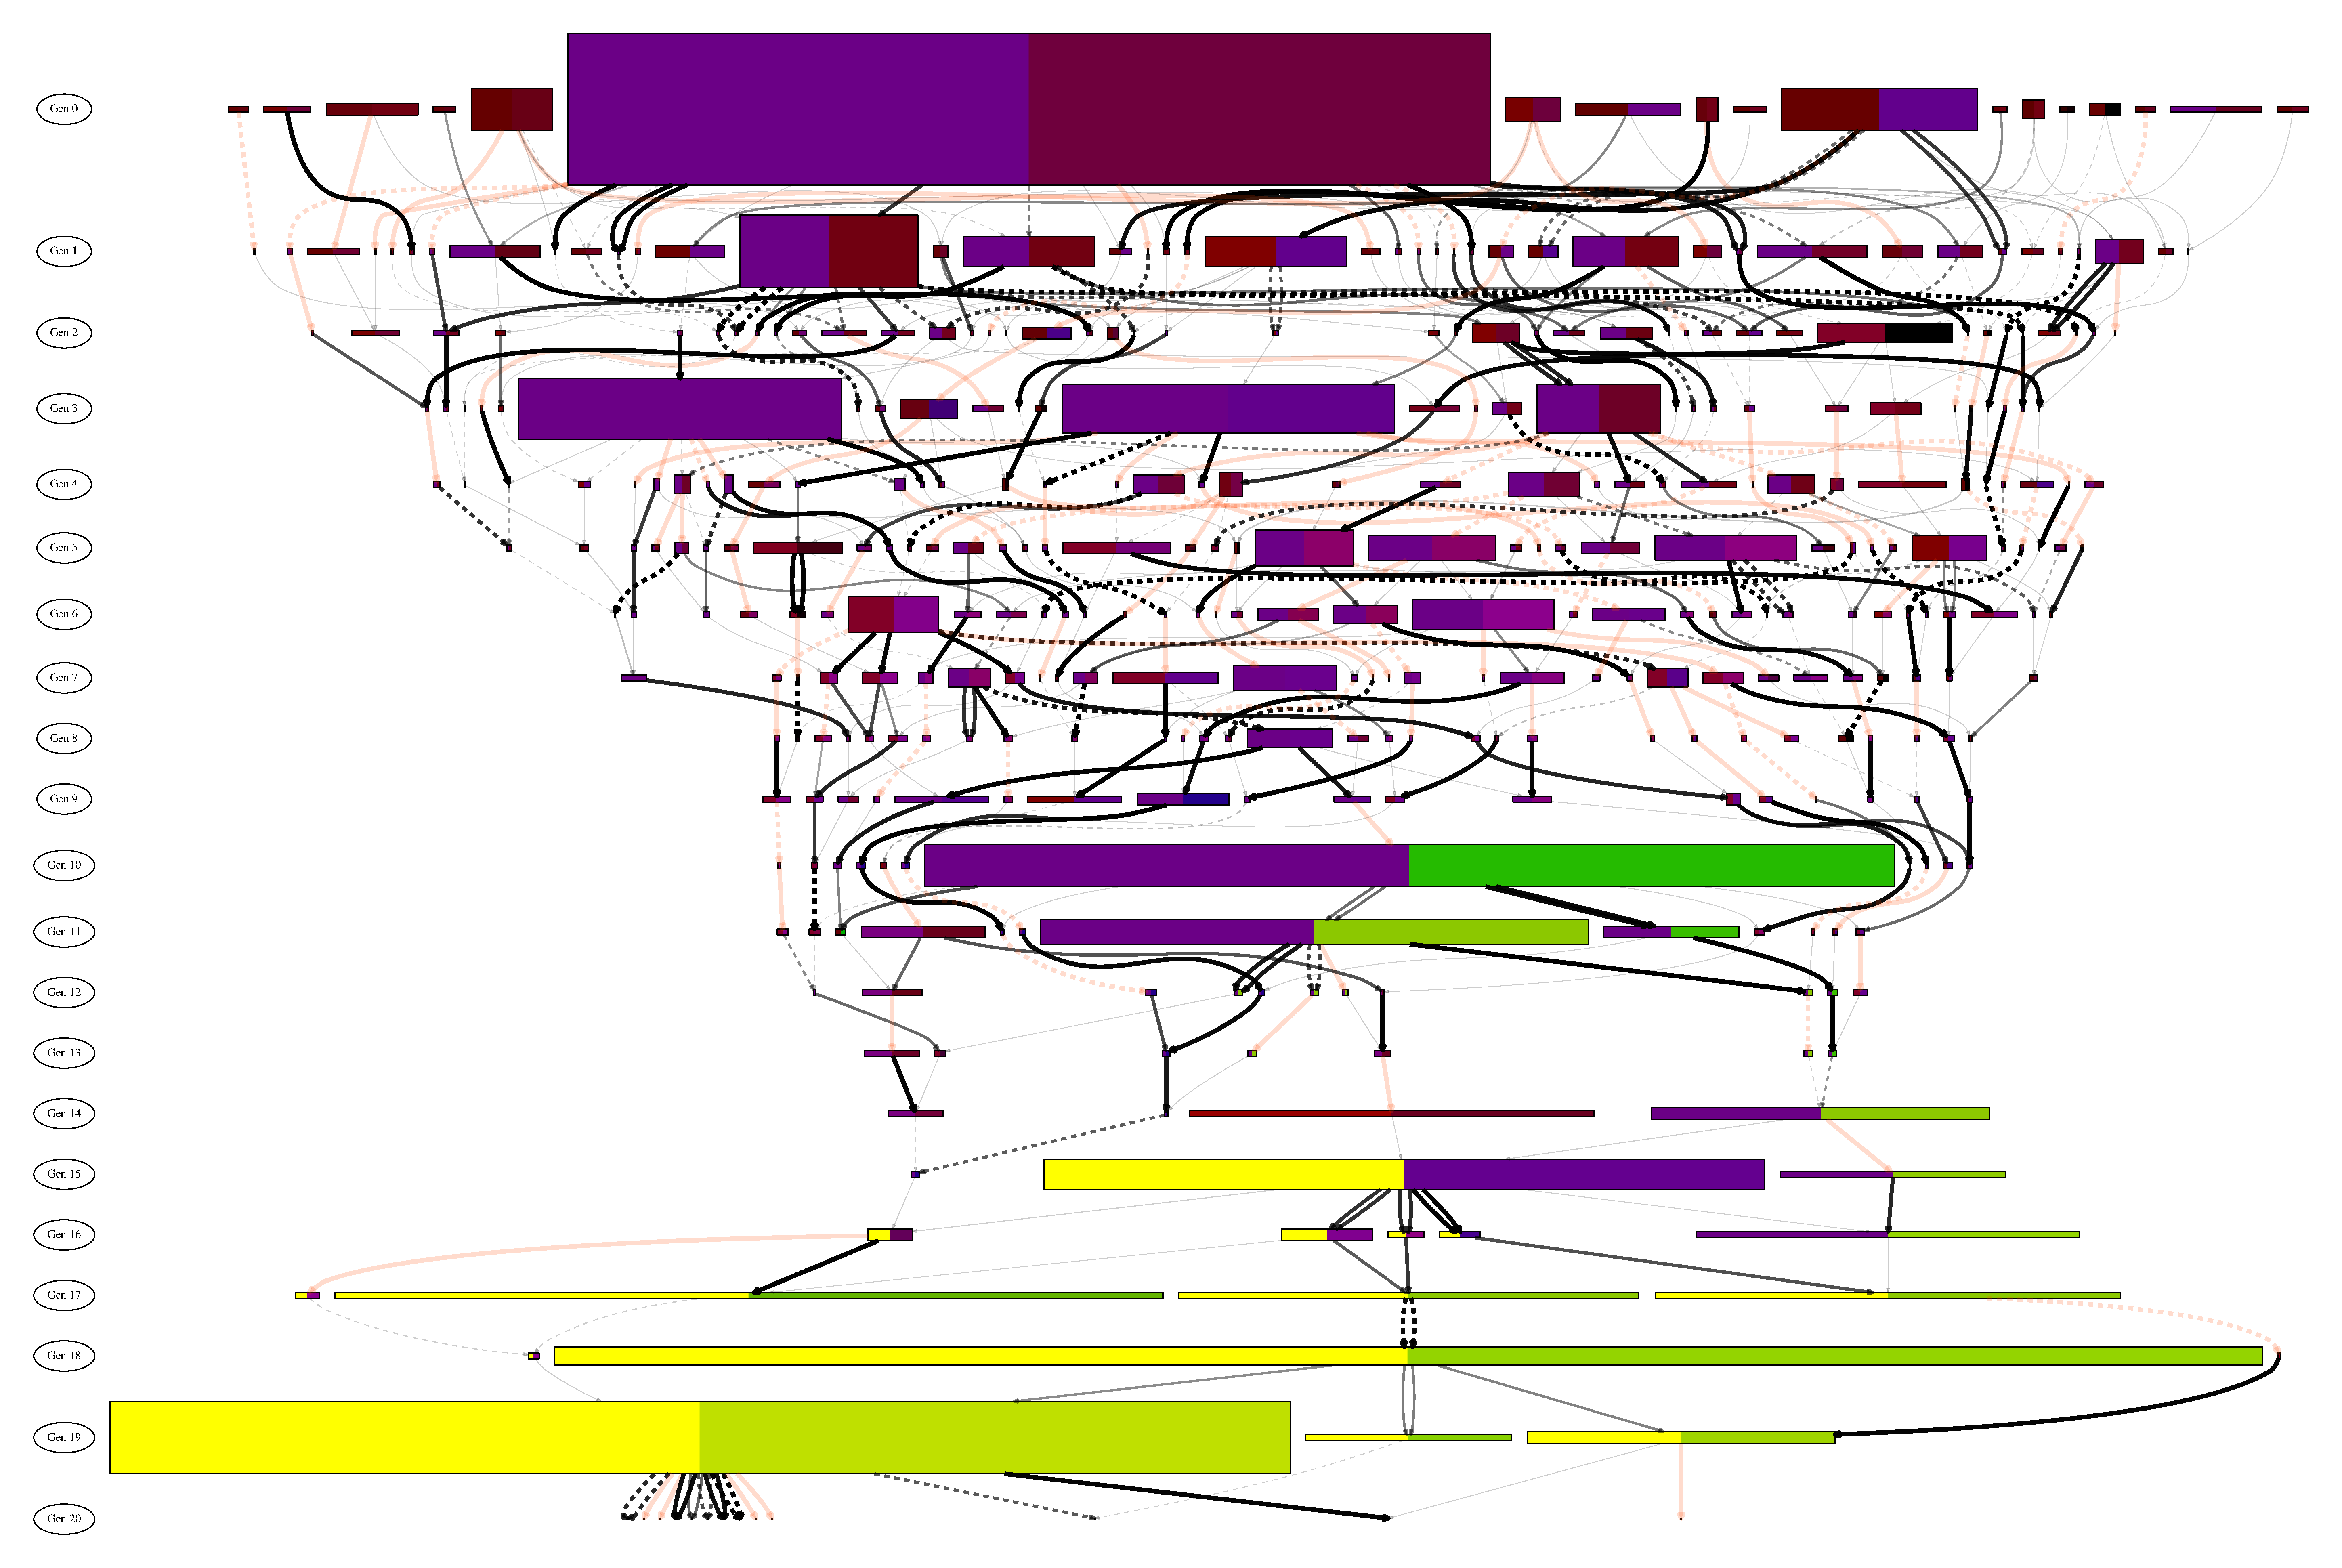
\includegraphics[width=\textwidth]{Illustrations/run0_bi_color_shaded_percent0.pdf}
\end{column}
\end{columns}
\end{frame}

\begin{frame}{RBM Node Coloring}
\begin{columns}
% Column 1
\begin{column}{.4\textwidth}
\begin{itemize}
\item RBM = Restricted Boltzmann Machines
\item Dimensionality Reduction Problem
\item 200 tests $\rightarrow$ 3 values
\end{itemize}
\center
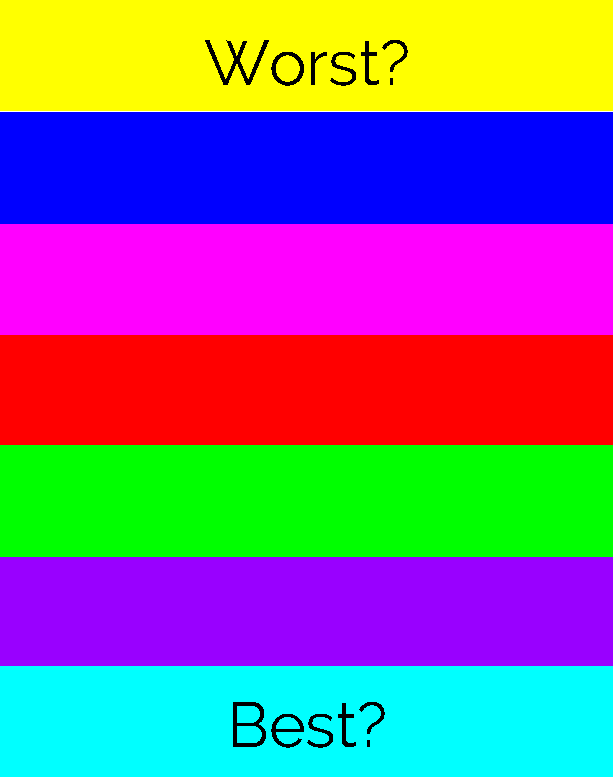
\includegraphics[height=0.4\textheight]{Illustrations/RBM.pdf}
\end{column}
% Column 2
\begin{column}{.6\textwidth}
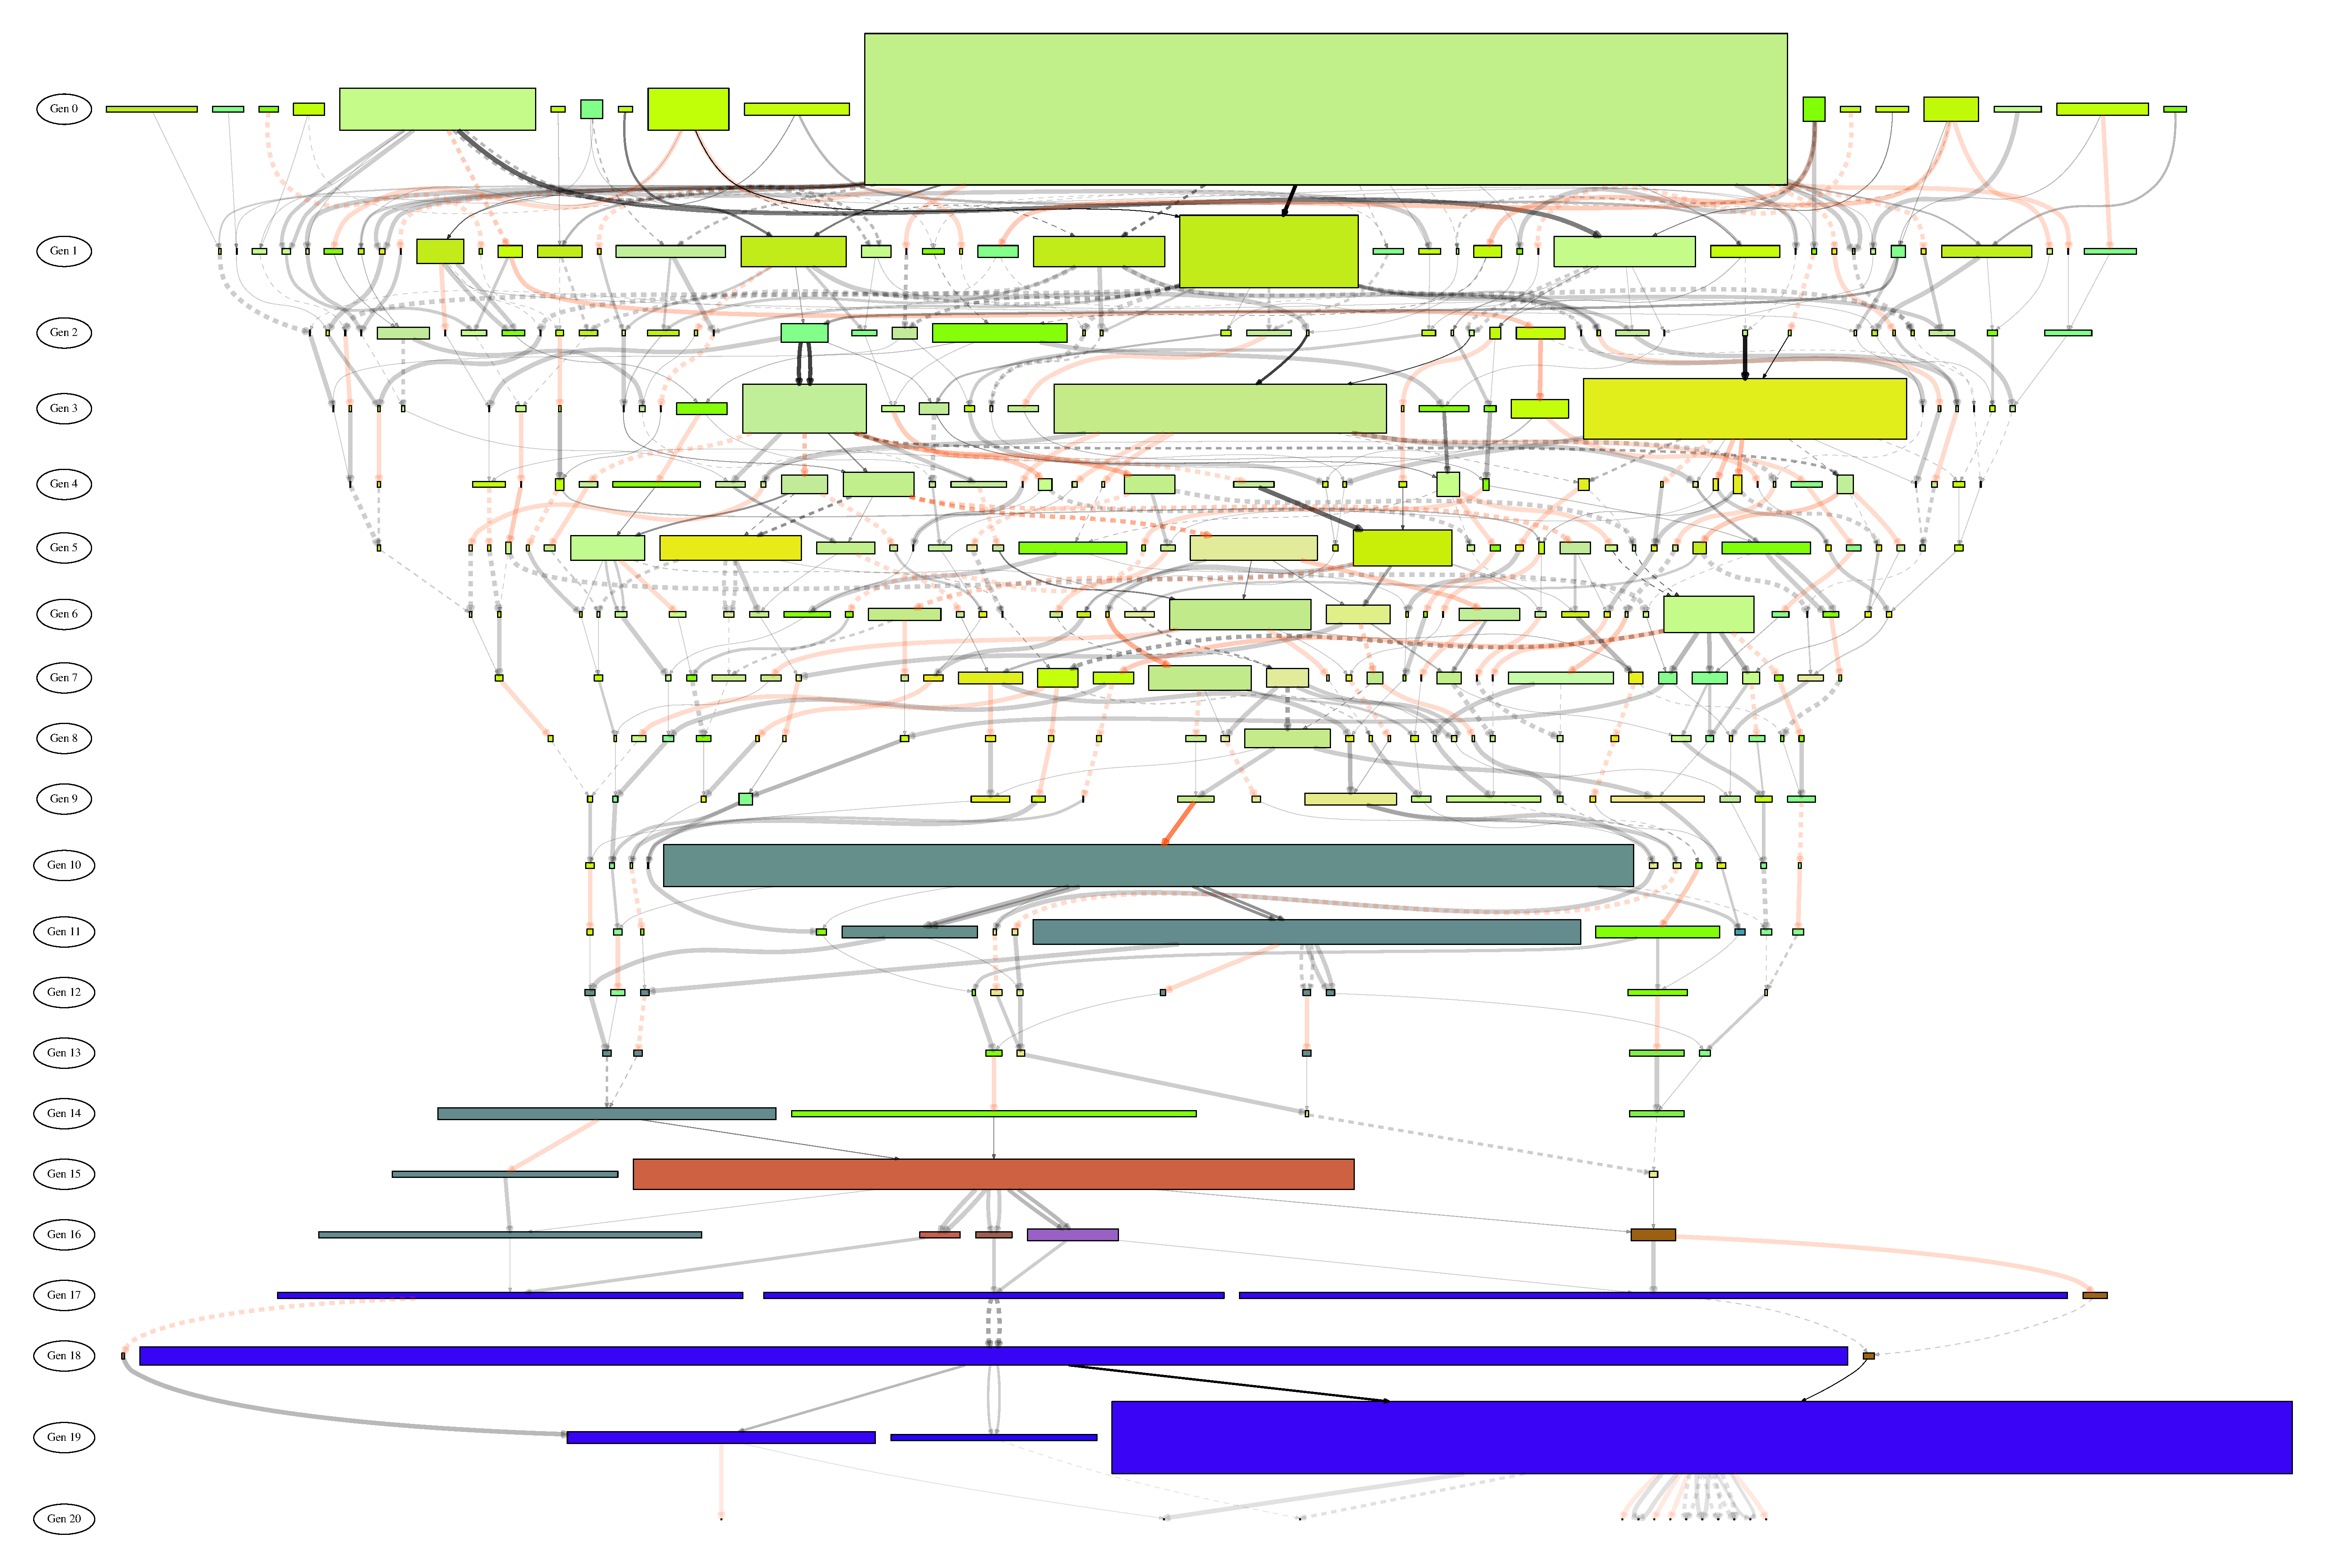
\includegraphics[width=\textwidth]{Illustrations/run0_RBM_color_full_30000.pdf}
\end{column}
\end{columns}
\end{frame}

\subsection[Edges]{Edges}

\begin{frame}{Edges}
Edges represent how an individual was created. \\
There are two main techniques: crossover and mutation.
\begin{itemize}
\item Crossover \\ Sections of \underline{both parents} are combined together. 
\item Mutation \\ \underline{One parent} is copied and some instructions are mutated.
\end{itemize} 
\end{frame}


\begin{frame}{Edge Coloring \& Style}
\begin{columns}
% Column 1
\begin{column}{.47\textwidth}
\begin{itemize}
\item Crossover is indicated by \underline{black} edges.
\item Mutation is indicated by \underline{\color{orange} orange}  edges.
\item Solid versus dashed is for variations of crossover and mutation.
\item Transparency is based on the number of children of the child.
\begin{itemize}
\item Transparent: Few Children
\item Opaque: Many Children
\end{itemize}
\end{itemize} 
\end{column}
% Column 2
\begin{column}{.6\textwidth}
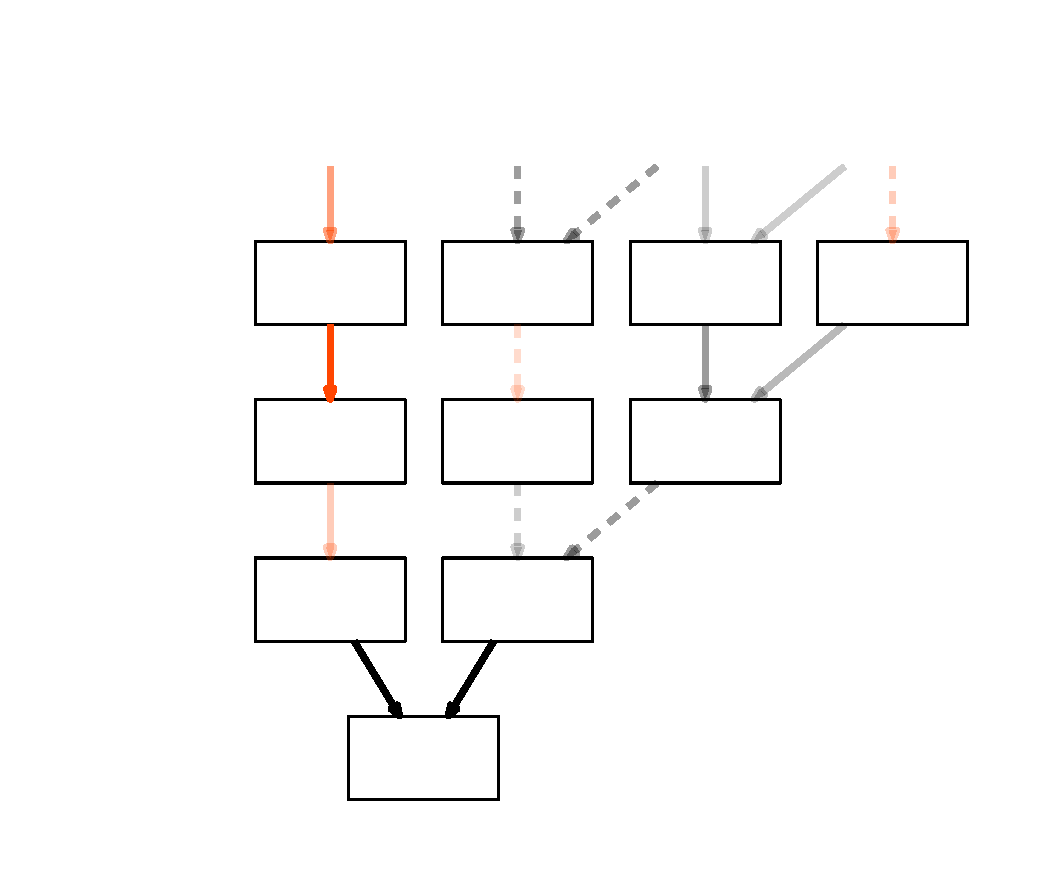
\includegraphics[width=\textwidth]{Illustrations/family_edges.pdf} 
\end{column}
\end{columns}
\end{frame}

\begin{frame}{Full Examples in RBM Coloring}
\begin{columns}
% Column 1
\begin{column}{.6\textwidth}
\center
\begin{itemize}
\item Run 0: Ends in 20 Generations
\item Run 1: Ends in 129 Generations
\begin{itemize}
\item Notice waist with large nodes
\end{itemize}
\end{itemize}
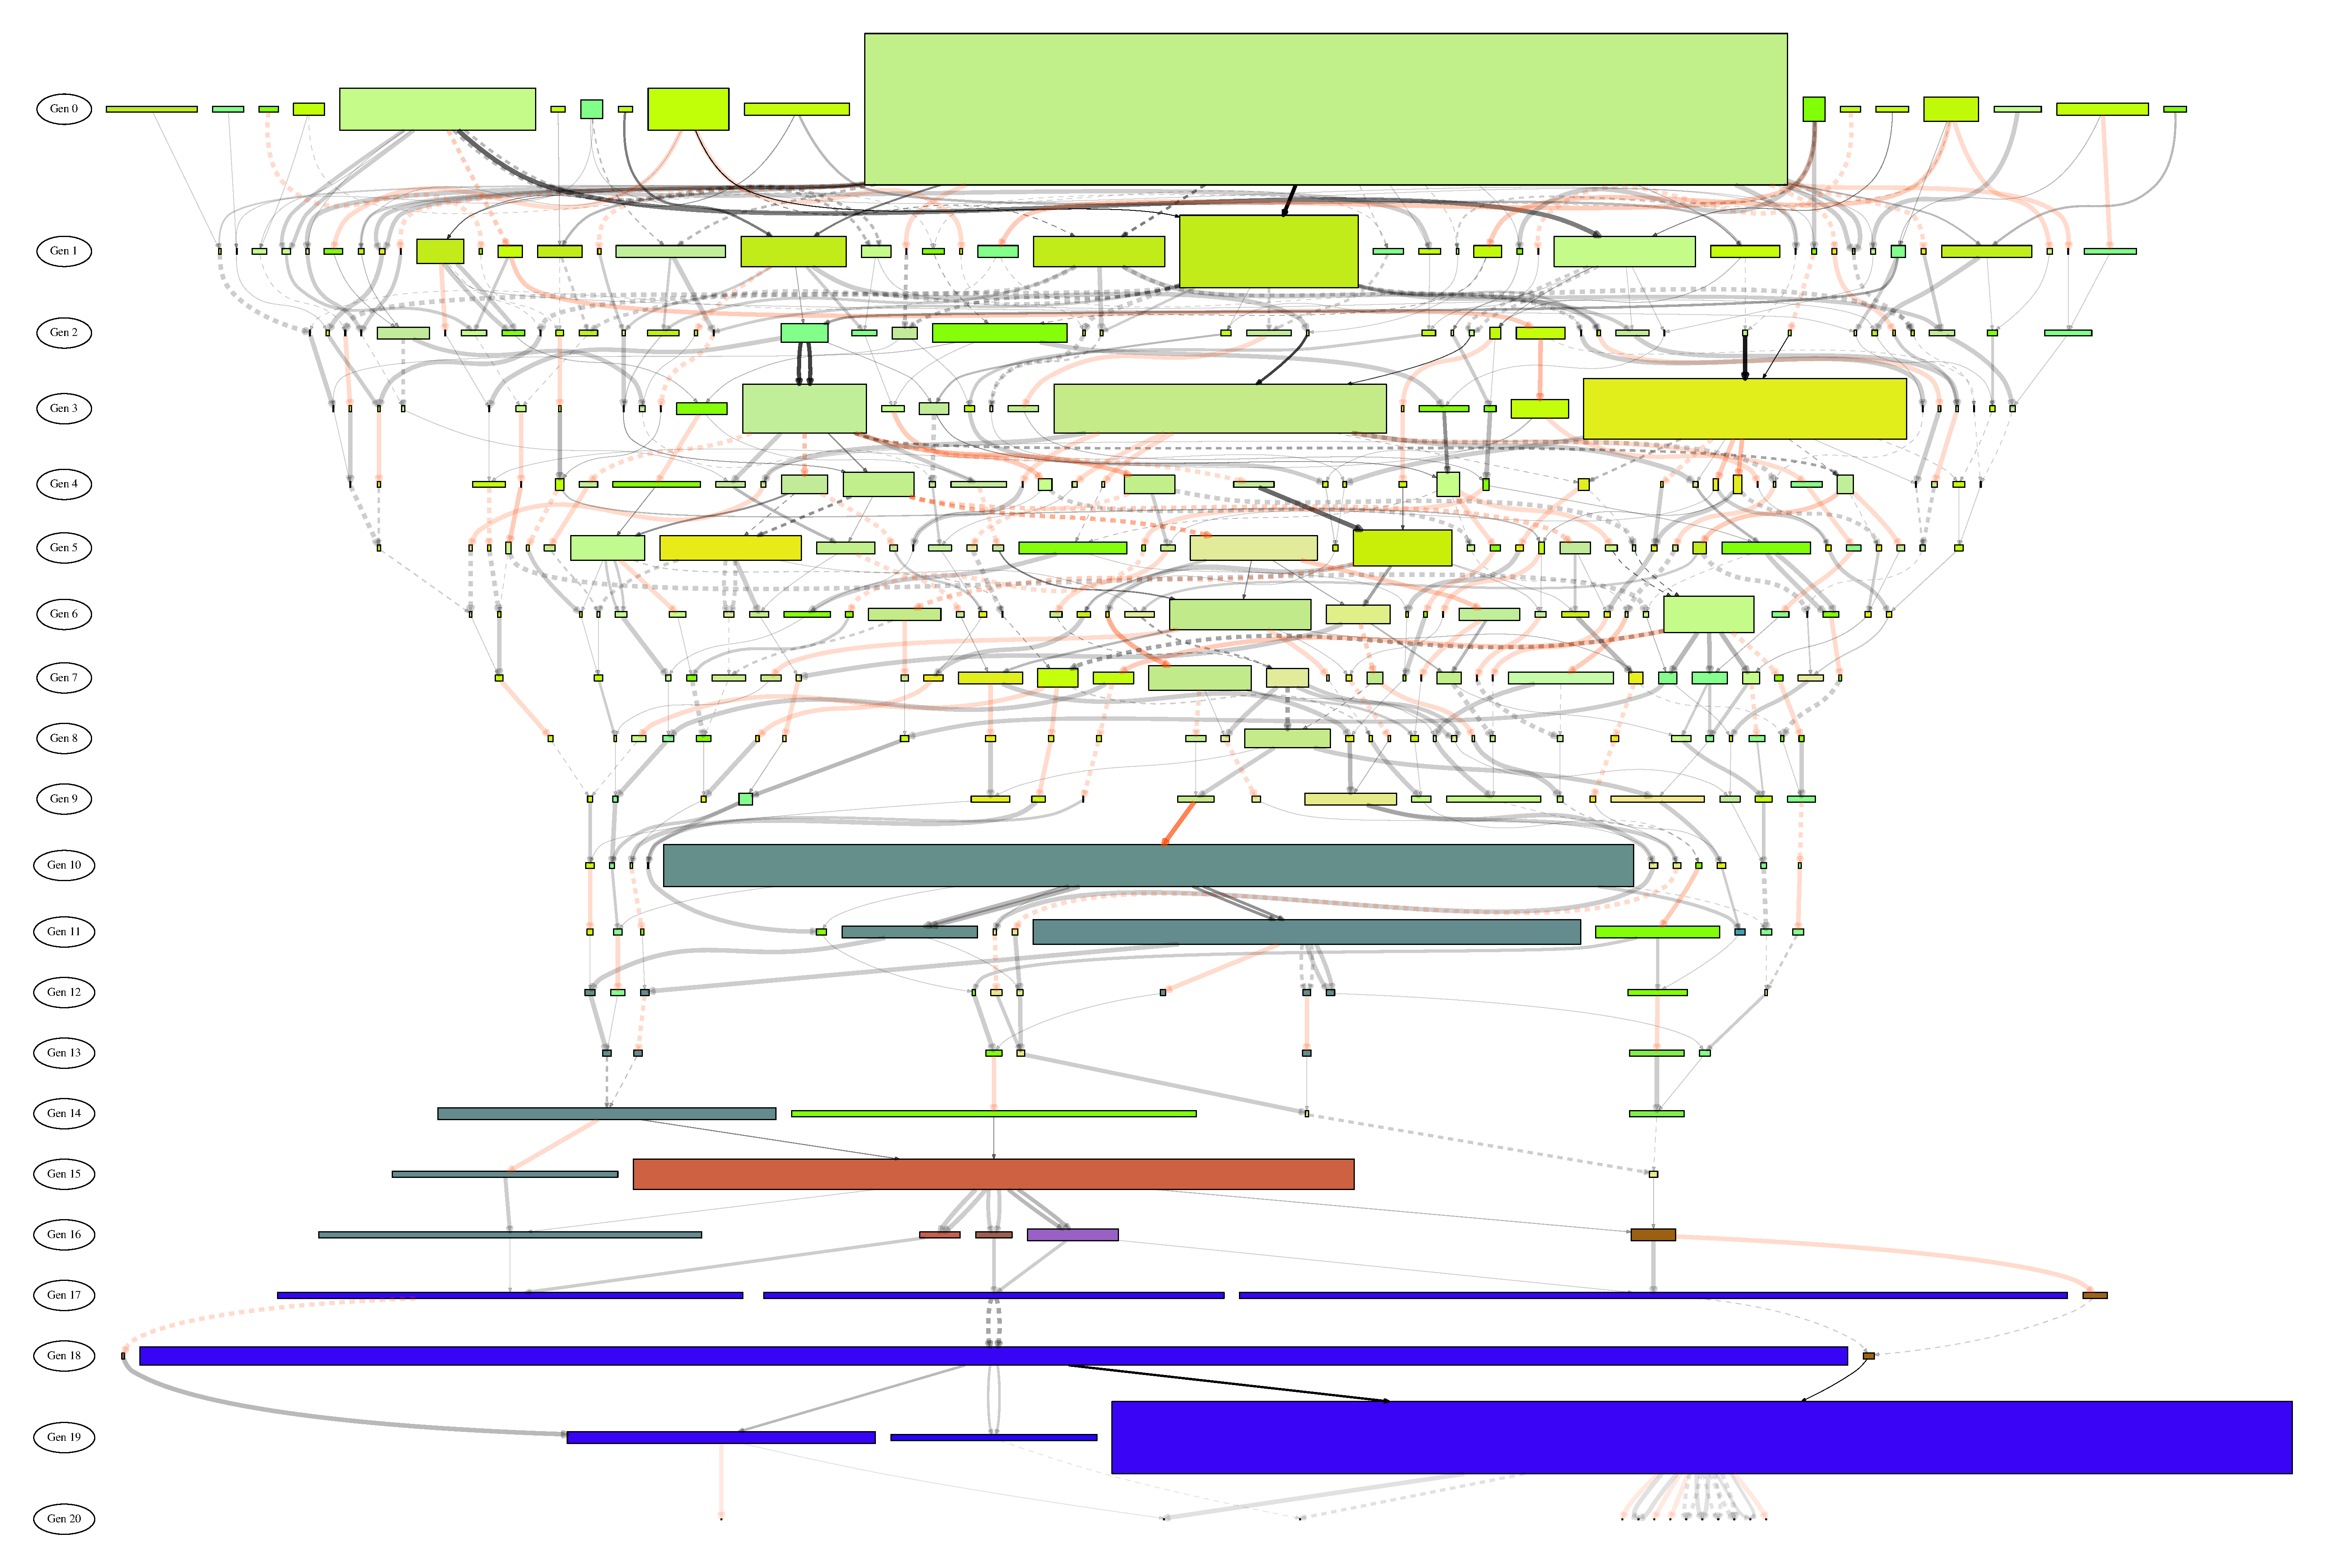
\includegraphics[width=\textwidth]{Illustrations/run0_RBM_color_full_30000.pdf} 
\end{column}
% Column 2
\begin{column}{.45\textwidth}
\center
\includegraphics[height=.85\textheight]{Illustrations/run1_RBM_small.pdf} 
\end{column}
\end{columns}
\end{frame}

%~~~~~~~~~~What did I learn?~~~~~~~~~~~~~~~~~~~~~~~~~~~~~~~~~~~~~~~~~~~~~~~~~~~~~~~~~~~~~~~~~~~~~~~~~~~~~~~~~~~~~~~

\section{What did I learn?}

\subsection{Hyperselection}
\begin{frame}{Hyperselection}
One focus of this research was to examine \textit{hyperselection}.
This occurs when an individual receives a noticeably high number selections in a population. 
\center 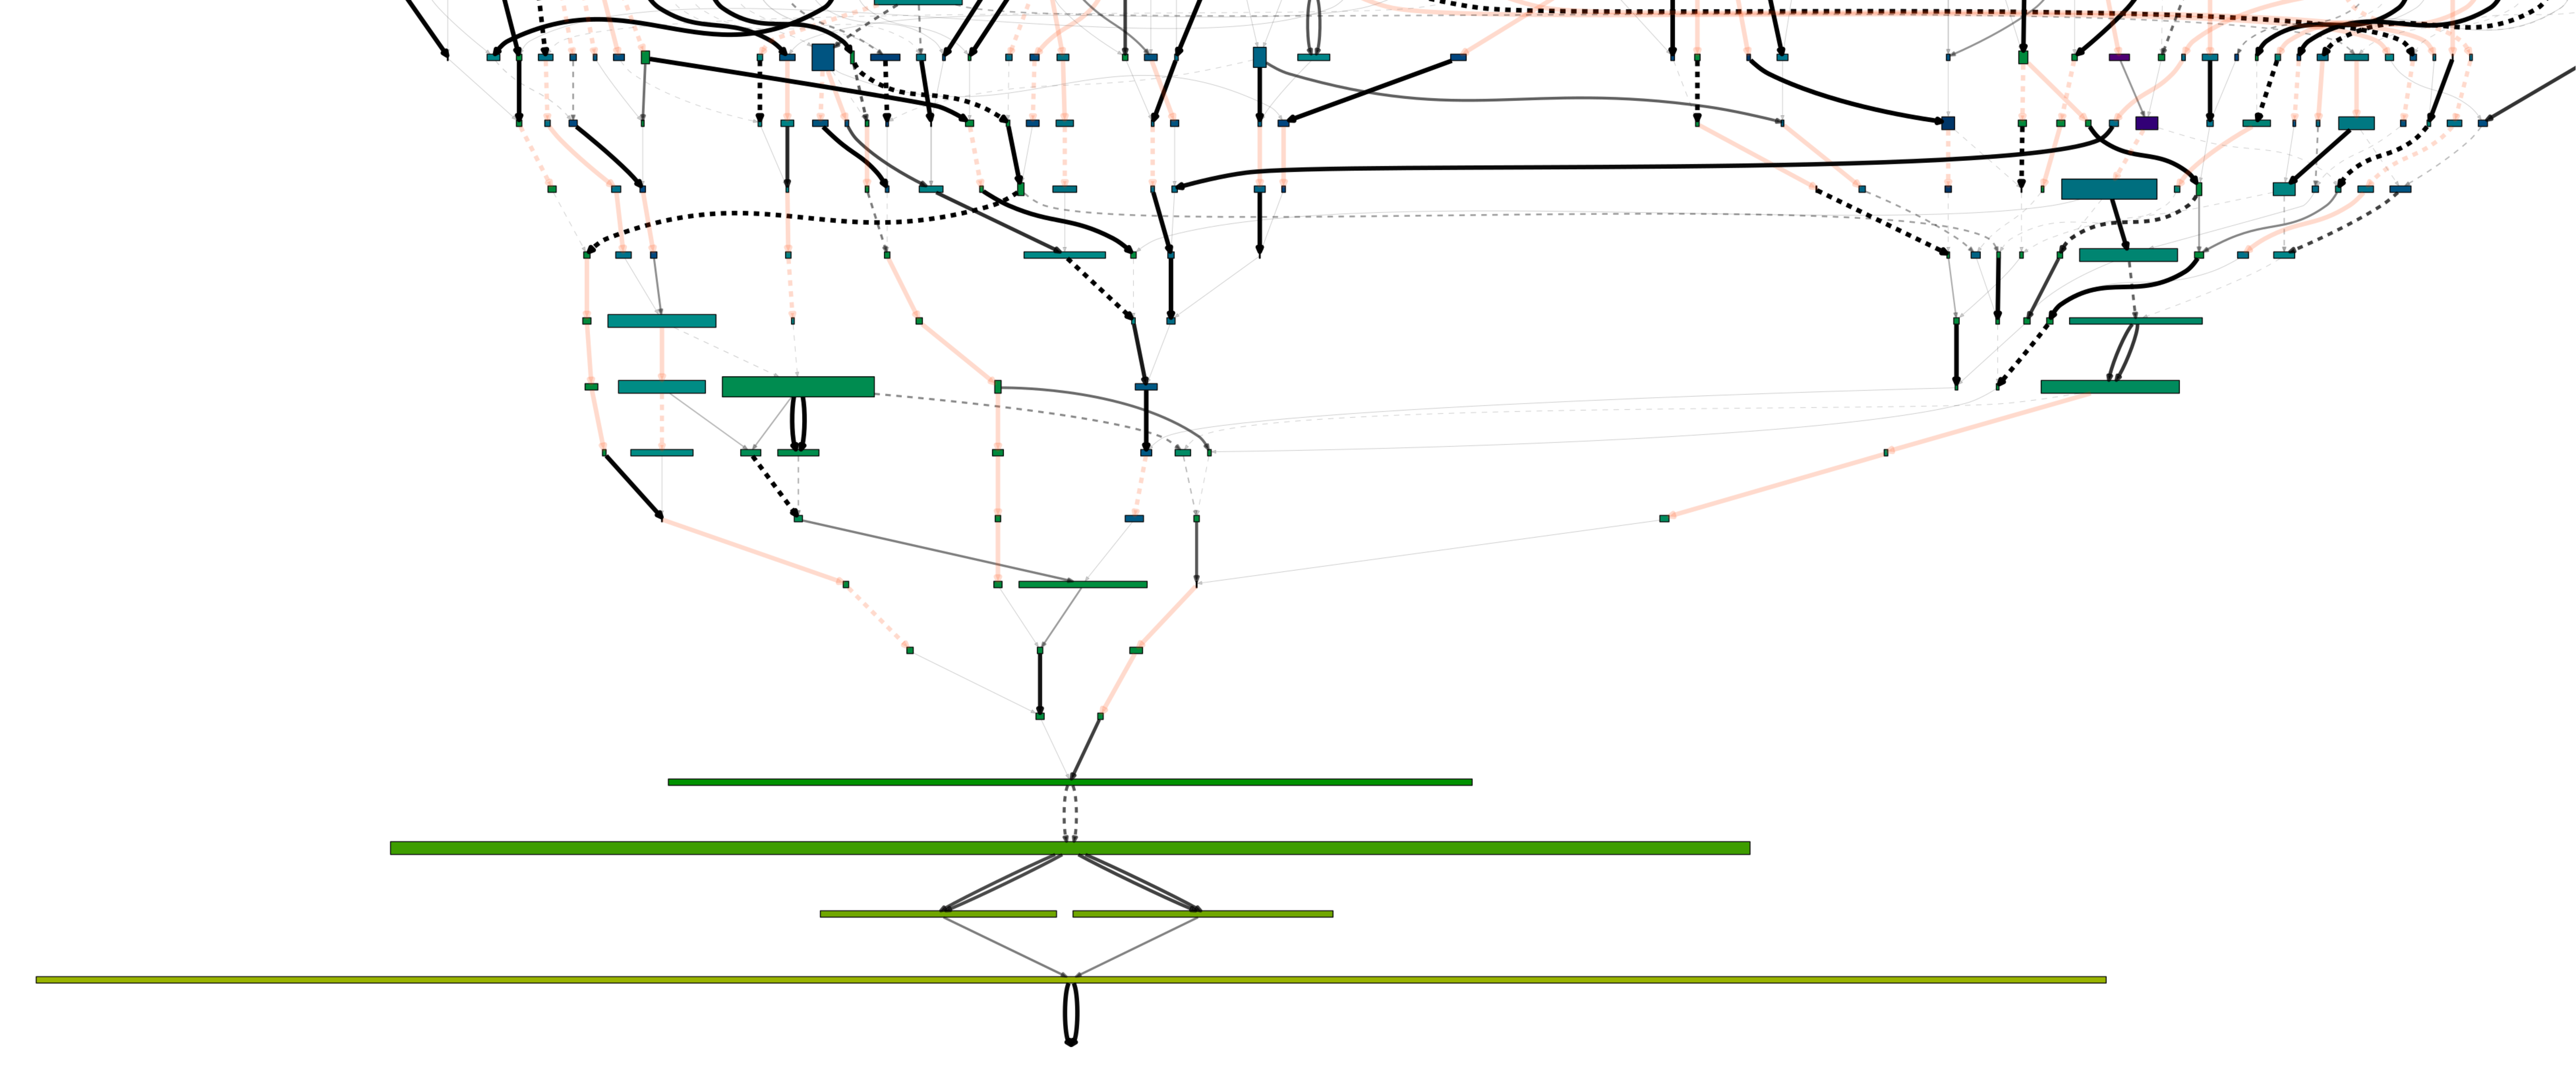
\includegraphics[width=\textwidth]{Illustrations/cropped.pdf} \\
In our graphs, we can see this as a \underline{very wide} node. 
\end{frame}

\subsection{Filtering Ancestry Trees}

\begin{frame}{Filtering Ancestry Trees}
\begin{columns}
% Column 1
\begin{column}{.6\textwidth}
\begin{itemize}
\item This is still a lot of data!
\begin{itemize}
\item 22,435 Individuals
\item 1,597 Individuals
\end{itemize}
\item We filter out parents who did not contribute much genetic information.
\item Numbers on edges indicate similarity.
\item The smaller the number is, the more similar they are.
\end{itemize}
\end{column}
% Column 2
\begin{column}{.45\textwidth}
\center
\includegraphics[height=.85\textheight]{Illustrations/run1_RBM_color_filtered_and_full_60000_2.pdf} 
\end{column}
\end{columns}
\end{frame}

\begin{frame}{Another Filtered Example}
\center
394 Individuals \hspace{4.5cm} 54 Individuals \\
\includegraphics[height=.8\textheight]{Illustrations/run0_RBM_color_both_runs_40.pdf} 
\end{frame}

\section{Conclusions}
\begin{frame}{Conclusions}
In Our Research We've:
\begin{itemize}
\item Turned our complex runs into organized ancestry trees.
\item Modified aspects of both nodes and edges to visualize analytics.
\item Learned about hyperselection and filtering ancestry trees.
\end{itemize}
\vspace{.5cm}
The Next Step:
\begin{itemize}
\item Presenting related work in May at GPTP in Ann Arbor, Michigan
\item In July we'll be attending GECCO in Denver, Colorado
\end{itemize}
\end{frame}

\begin{frame}{Thanks!}
\center \Large
Thank you for your time \& attention! \\ \medskip
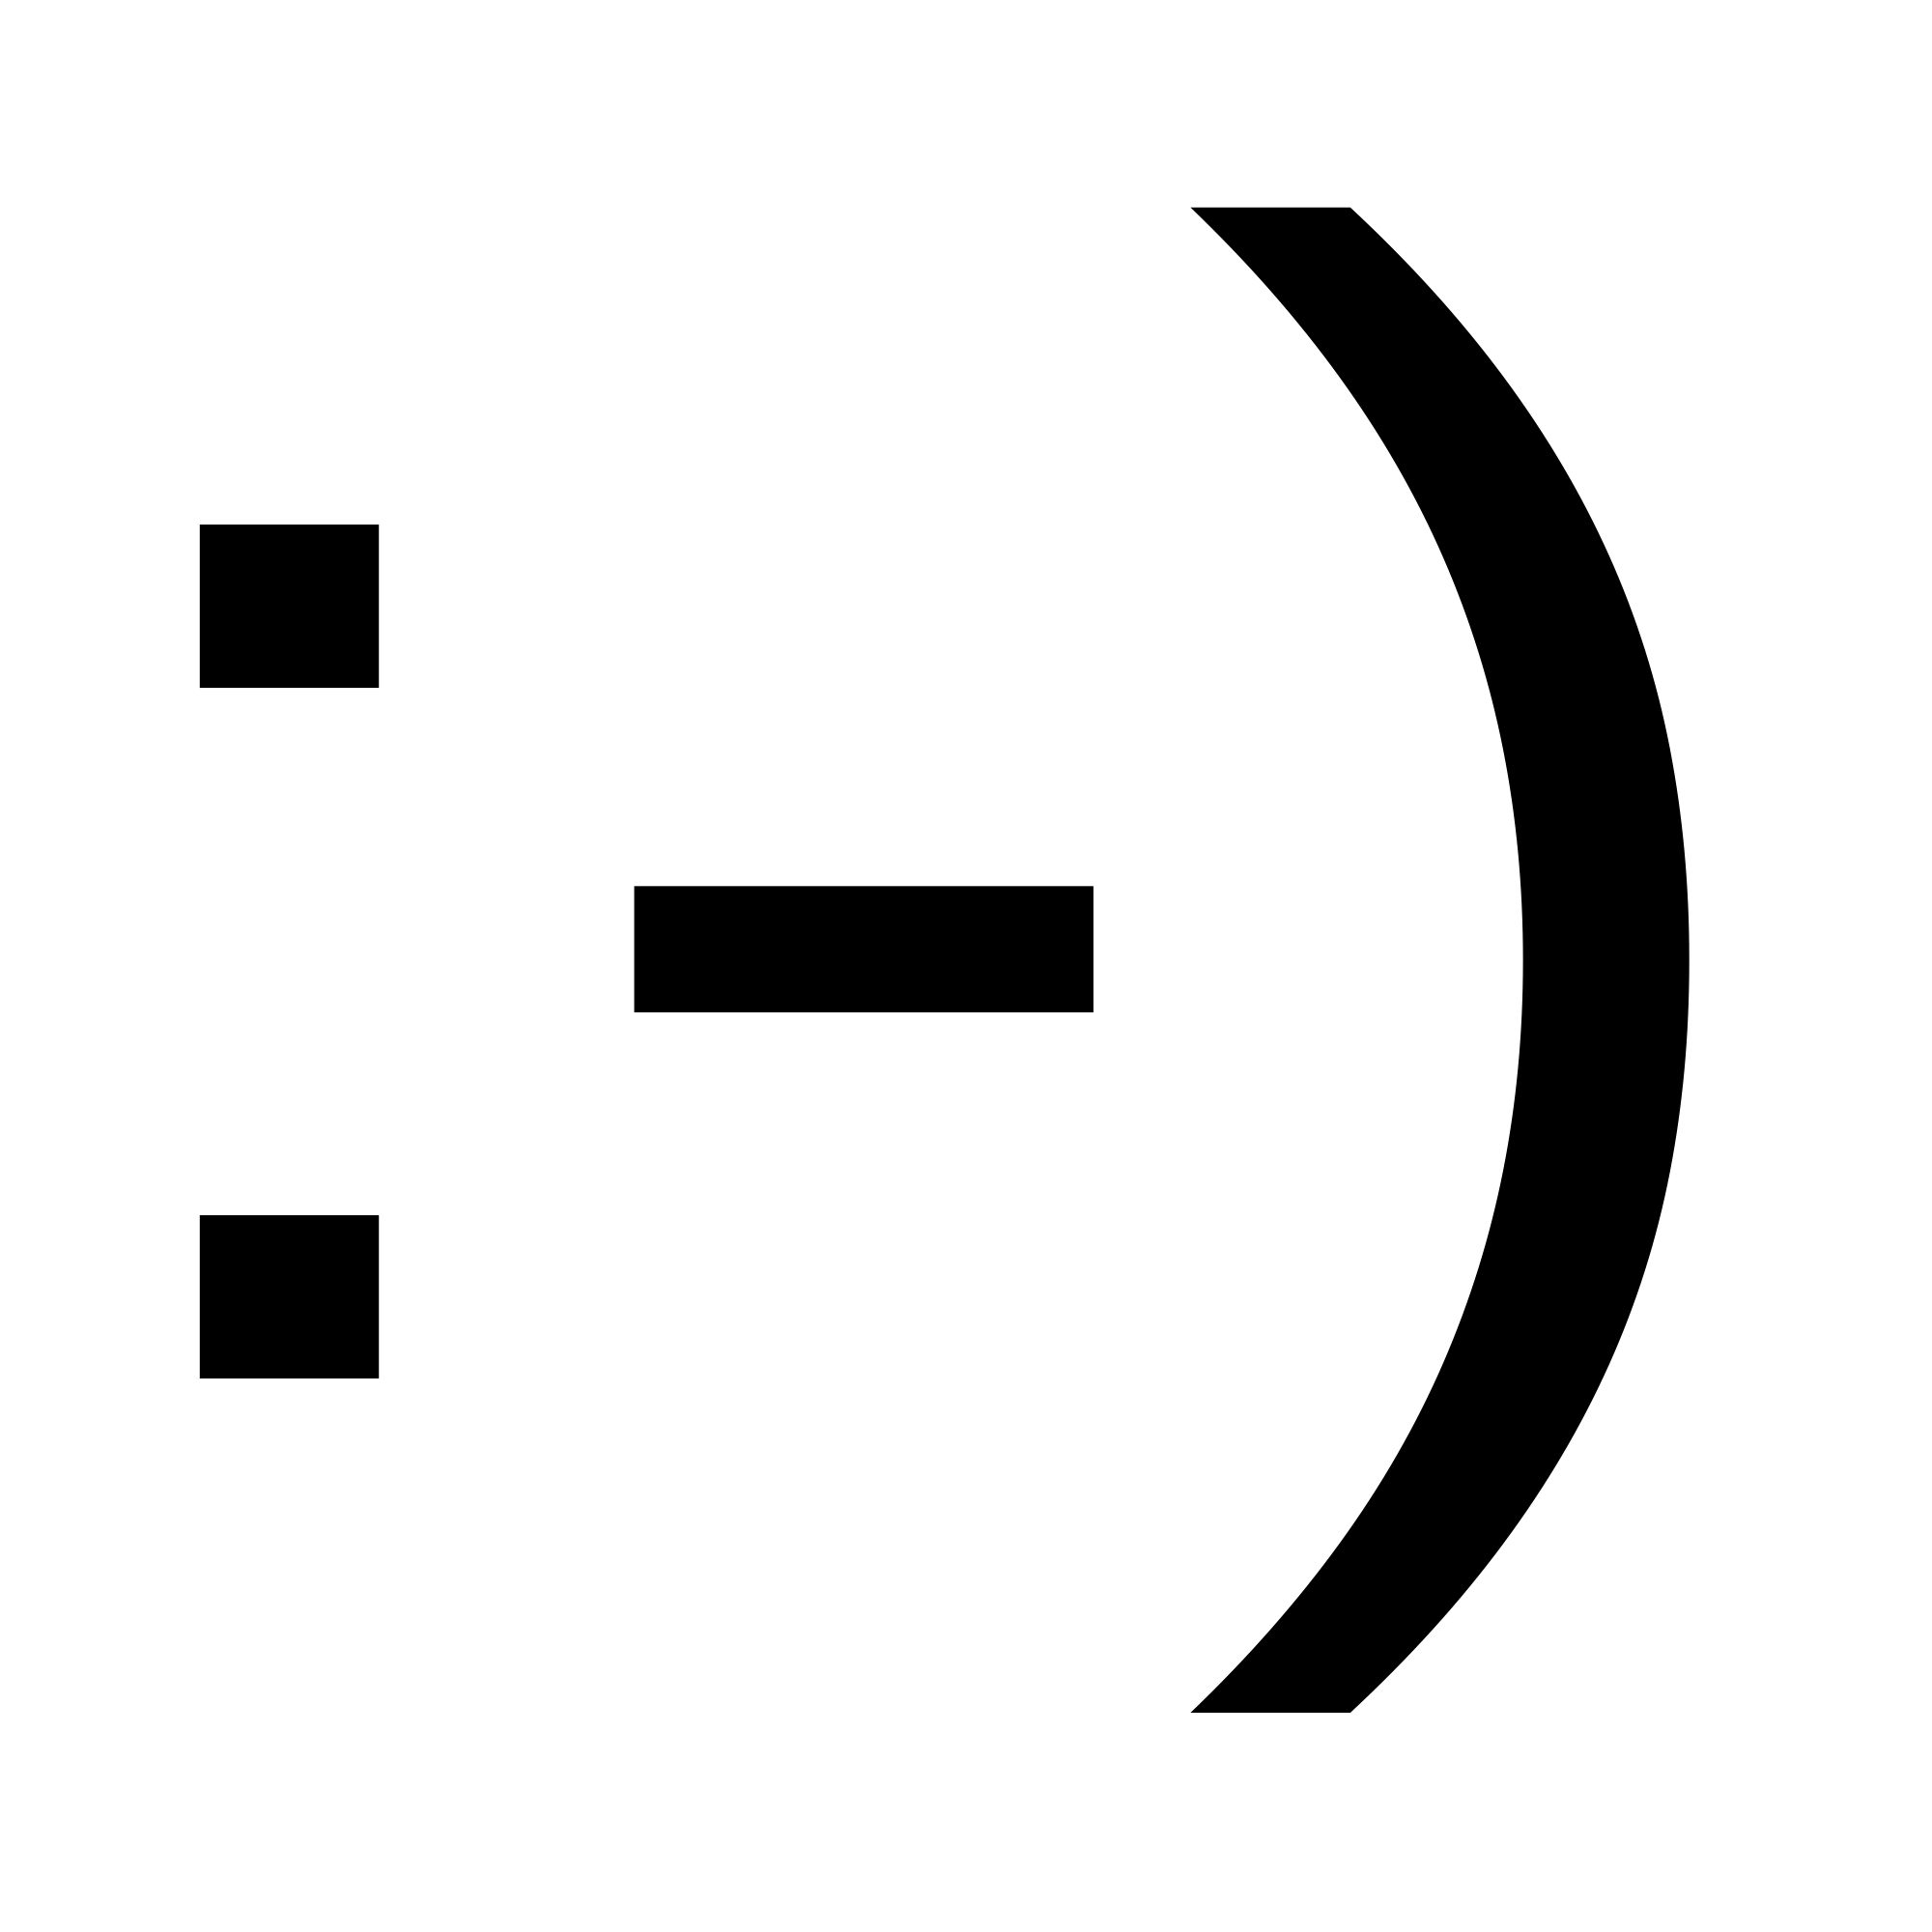
\includegraphics[width=.2\textwidth]{Illustrations/smile.png} \\ \medskip
Special Thanks to Nic McPhee!  
\end{frame}

%~~~~~~~~~~References~~~~~~~~~~~~~~~~~~~~~~~~~~~~~~~~~~~~~~~~~~~~~~~~~~~~~~~~~~~~~~~~~~~~~~~~~~~~~~~~~~~~~~~

\section*{References}

\begin{frame} 
	\frametitle{References} 
	
	\begin{thebibliography}{lskdjf}
	\small 
	\bibitem{Burlacu:2013:GECCOcomp:new}
B.~Burlacu, M.~Affenzeller, M.~	Kommenda, S.~Winkler, and G.~Kronberger.
\newblock Visualization of genetic lineages and inheritance
information in genetic programming.
\newblock In Christian Blum, \emph{et al}, editors, {\em GECCO '13}, pages 1351--1358, New York, NY, USA, 2013.
	
	\bibitem{hyper:2016}
	T.~Helmuth, N.~F.~McPhee, and L.~Spector.
\newblock The Impact of Hyperselection on Lexicase Selection.
\newblock {\em GECCO '16}, Denver, CO, USA 2016.
  
	\bibitem{vis:2016}
	N.~F.~McPhee, M.~Casale, M.~Finzel, T.~Helmuth, and L.~Spector.
\newblock Visualizing genetic programming ancestries using graph databases.
\newblock {\em GECCO '16}, Denver, CO, USA 2016.
	
	\bibitem{gptp:2016}
	N.~F.~McPhee, M.~Finzel, M.~Casale, T.~Helmuth, and L.~Spector.
\newblock A detailed analysis of a PushGP run.
\newblock (Forthcoming) {\em GPTP '16}, Ann Arbor, MI, USA 2016.
	

  
  	\end{thebibliography}
	
\end{frame} 

\end{document}


